%! TeX program = lualatex
\documentclass[a4paper,12pt,article]{memoir}

% TeX root=../main.tex

\settrimmedsize{\stockheight}{\stockwidth}{*}
\settypeblocksize{220mm}{130mm}{*}
\setlrmargins{*}{*}{1.7}
\setulmargins{30mm}{*}{*}
\setmarginnotes{20pt}{100pt}{10pt}
\checkandfixthelayout%

% \setsidefeet{\marginparsep}{\marginparwidth}%
% {0.8\onelineskip}{0pt}%
% {\normalfont\footnotesize}{\textheight}%
\setsidecaps{\marginparsep}{\marginparwidth}
\setlength{\footmarkwidth}{0.5em}
\setlength{\footmarksep}{0em}
\setlength{\footparindent}{0em}
\footmarkstyle{\textsuperscript{#1}\hspace{0.5em}}

\makeoddfoot{plain}{}{}{\thepage}
\makeevenfoot{plain}{\thepage}{}{}
\makepagestyle{ruled}
\makeevenfoot{ruled}{\thepage}{}{} % page numbers at the outside
\makeoddfoot{ruled}{}{}{\thepage}
\makeheadrule{ruled}{\textwidth}{0.75pt}
\makeevenhead{ruled}{\scshape\leftmark}{}{}
\makeoddhead{ruled}{}{}{\scshape\rightmark}
\makepsmarks{ruled}{%
	\nouppercaseheads%
	\createmark{chapter}{left}{shownumber}{\scshape}{.\space}
	\createmark{part}{right}{shownumber}{}{.\space}
	\createmark{section}{right}{shownumber}{}{.\space}
	\createmark{subsection}{right}{shownumber}{}{.\space}
	\createplainmark{toc}{both}{\contentsname}
	\createplainmark{lof}{both}{\listfigurename}
	\createplainmark{lot}{both}{\listtablename}
	\createplainmark{bib}{both}{\bibname}
	\createplainmark{index}{both}{\indexname}
	\createplainmark{glossary}{both}{\glossaryname}
}

% decorando divisões
\setsecnumdepth{subsection}
\setcounter{tocdepth}{3}
\newcommand\chap[1]{%
	\chapter*[#1]{#1}%
	\addcontentsline{toc}{chapter}{#1}}


% paleta de cores
\usepackage{xcolor}
\definecolor{green}{rgb}{16,87,87} % rgb(16,87,87)
\definecolor{red}{rgb}{193, 11, 105} % rgb(193, 11, 105)
\definecolor{yellow}{rgb}{218,222,104} % rgb(218,222,104)
\definecolor{pink}{rgb}{243,179,145} % rgb(243,179,145)
\definecolor{blue}{rgb}{161,184,206} % rgb(161,184,206)

\usepackage[tracking=true]{microtype}

\usepackage{scalefnt}


\usepackage[normalem]{ulem}
\usepackage{amsmath}
\usepackage[defblank]{paralist}
\usepackage{graphicx}
\usepackage{subcaption}
\usepackage{linguex}
\usepackage{multicol}
\usepackage{multirow}
\usepackage{tabto}

\usepackage{hyperref}
\hypersetup{%
	colorlinks=true, % false: boxed links; true: colored links
	linkcolor=green,  % color of internal links
	citecolor=green,  % color of links to bibliography
	filecolor=pink,  % color of file links
	urlcolor=green,
}
% Configurações para o autoref
\renewcommand{\figureautorefname}{Figura}
\renewcommand{\tableautorefname}{Tabela}
\renewcommand{\sectionautorefname}{Seção}
\renewcommand{\chapterautorefname}{Capítulo}
\renewcommand{\subsectionautorefname}{Subseção}


\directlua{dofile('./utils/pie.lua')}
\newcommand{\hittitetrans}[1]{%
  \directlua{hittite_transcription("#1")}}
\newcommand{\luwiantrans}[1]{%
  \directlua{luwian_transcription("#1")}}
\newcommand{\pietrans}[1]{%
  \directlua{pie_transcription("#1")}}

\newcommand{\Prep}{{\footnotesize\textsc{Prep.}}}
\newcommand{\Det}{{\footnotesize\textsc{Det.}}}
\newcommand{\Clt}{{\footnotesize\textsc{Clt.}}}
\newcommand{\Nom}{{\footnotesize\textsc{Nom.}}}
\newcommand{\Acu}{{\footnotesize\textsc{Acu.}}}
\newcommand{\Dat}{{\footnotesize\textsc{Dat.}}}
\newcommand{\Gen}{{\footnotesize\textsc{Gen.}}}
\newcommand{\Abl}{{\footnotesize\textsc{Abl.}}}
\newcommand{\Sg}{{\footnotesize\textsc{Sg.}}}
\newcommand{\Pl}{{\footnotesize\textsc{Pl.}}}
\newcommand{\Com}{{\footnotesize\textsc{Com.}}}
\newcommand{\Neut}{{\footnotesize\textsc{Neut.}}}
\newcommand{\Rel}{{\footnotesize\textsc{Rel.}}}
\newcommand{\Conj}{{\footnotesize\textsc{Conj.}}}
\newcommand{\Pret}{{\footnotesize\textsc{Pret.}}}
\newcommand{\Pro}{{\footnotesize\textsc{Pro.}}}
\newcommand{\Refl}{{\footnotesize\textsc{Refl.}}}
\newcommand{\La}[1]{\textsc{l}.#1}
\newcommand{\logo}[1]{\textnormal{#1}}
\newcommand{\spac}{\textsuperscript{\textnormal{I}}}
\newcommand{\lmasc}{\textnormal{|}}
\newcommand{\Isep}{\textsuperscript{I}}
\newcommand{\luwmasc}{{\textsuperscript{𔖶}}}
\newcommand{\lbreak}{\hspace{2pt}\textnormal{||}\hspace{2pt}}
\newcommand{\ipa}[1]{\foreignlanguage{ipa}{#1}}
\newcommand{\pie}{\textsc{pie}}
\newcommand{\pac}{\textsc{pac}}
\newcommand{\parnumr}[2]{#1 \Roman{parcount}}
\newcommand{\parnuma}[2]{#1 \arabic{parcount}}
\newcounter{parcount}
\newenvironment{parnumbersa}[1][§]{%
   \par%
	 \everypar{\hangpara{3em}{1}\stepcounter{parcount} \textnormal{\normalsize\parnuma{#1}}
	 \tabto{2em}}%
}{}
\newenvironment{parnumbersr}[2][§]{%
   \par%
	 \everypar{\hangpara{3em}{1}\stepcounter{parcount} \textnormal{\normalsize\parnumr{#1}}
	 \tabto{2em}}%
}{}

\usepackage{csquotes}
\usepackage{fontspec}
\usepackage[main=brazil, bidi=basic]{babel}
\defaultfontfeatures{Renderer=Harfbuzz}

\babelfont[brazil]{rm}[
	SmallCapsFont=Gentium Plus,
	SmallCapsFeatures={Letters=SmallCaps}]{Crimson Pro}
\babelfont[brazil]{sf}{Noto Sans}
\babelfont[brazil]{tt}[Scale=0.8]{Mononoki Nerd Font}

\babelfont[german]{rm}[
	SmallCapsFont=Gentium Plus,
	SmallCapsFeatures={Letters=SmallCaps}]{Crimson Pro}
\babelfont[brazil]{sf}{Noto Sans}
\babelfont[brazil]{tt}[Scale=0.8]{Mononoki Nerd Font}

\babelfont[english]{rm}[
	SmallCapsFont=Gentium Plus,
	SmallCapsFeatures={Letters=SmallCaps}]{Crimson Pro}
\babelfont[english]{sf}{Noto Sans}
\babelfont[english]{tt}[Scale=0.8]{Mononoki Nerd Font}

\babelfont[german]{rm}[
	SmallCapsFont=Gentium Plus,
	SmallCapsFeatures={Letters=SmallCaps}]{Crimson Pro}
\babelfont[german]{sf}{Noto Sans}
\babelfont[german]{tt}[Scale=0.8]{Mononoki Nerd Font}


\babelprovide[import, onchar=ids fonts letters]{ancientgreek}
\babelfont[ancientgreek]{rm}{Brill}
\babeltags{grc = ancientgreek}

\babelprovide[import]{hebrew}
\babelfont[hebrew]{rm}[Scale=0.8]{Ezra SIL}

\babelprovide[onchar=ids fonts]{luwian}
\babelfont[luwian]{rm}[
	SmallCapsFont=Gentium Plus,
Script=Anatolian Hieroglyphs]{Noto Sans Anatolian Hieroglyphs}
\babelfont[luwian]{sf}[
	SmallCapsFont=Gentium Plus,
Script=Anatolian Hieroglyphs]{Noto Sans Anatolian Hieroglyphs}
\babelcharproperty{`𔐀}{locale}{luwian}
\babelcharproperty{`𔐁}{locale}{luwian}
\babelcharproperty{`𔐂}{locale}{luwian}
\babelcharproperty{`𔐃}{locale}{luwian}
\babelcharproperty{`𔐄}{locale}{luwian}
\babelcharproperty{`𔐅}{locale}{luwian}
\babelcharproperty{`𔐆}{locale}{luwian}
\babelcharproperty{`𔐇}{locale}{luwian}
\babelcharproperty{`𔐈}{locale}{luwian}
\babelcharproperty{`𔐉}{locale}{luwian}
\babelcharproperty{`𔐊}{locale}{luwian}
\babelcharproperty{`𔐋}{locale}{luwian}
\babelcharproperty{`𔐌}{locale}{luwian}
\babelcharproperty{`𔐍}{locale}{luwian}
\babelcharproperty{`𔐎}{locale}{luwian}
\babelcharproperty{`𔐏}{locale}{luwian}
\babelcharproperty{`𔐐}{locale}{luwian}
\babelcharproperty{`𔐑}{locale}{luwian}
\babelcharproperty{`𔐒}{locale}{luwian}
\babelcharproperty{`𔐓}{locale}{luwian}
\babelcharproperty{`𔐔}{locale}{luwian}
\babelcharproperty{`𔐕}{locale}{luwian}
\babelcharproperty{`𔐖}{locale}{luwian}
\babelcharproperty{`𔐗}{locale}{luwian}
\babelcharproperty{`𔐘}{locale}{luwian}
\babelcharproperty{`𔐙}{locale}{luwian}
\babelcharproperty{`𔐚}{locale}{luwian}
\babelcharproperty{`𔐛}{locale}{luwian}
\babelcharproperty{`𔐜}{locale}{luwian}
\babelcharproperty{`𔐝}{locale}{luwian}
\babelcharproperty{`𔐞}{locale}{luwian}
\babelcharproperty{`𔐟}{locale}{luwian}
\babelcharproperty{`𔐠}{locale}{luwian}
\babelcharproperty{`𔐡}{locale}{luwian}
\babelcharproperty{`𔐢}{locale}{luwian}
\babelcharproperty{`𔐣}{locale}{luwian}
\babelcharproperty{`𔐤}{locale}{luwian}
\babelcharproperty{`𔐥}{locale}{luwian}
\babelcharproperty{`𔐦}{locale}{luwian}
\babelcharproperty{`𔐧}{locale}{luwian}
\babelcharproperty{`𔐨}{locale}{luwian}
\babelcharproperty{`𔐩}{locale}{luwian}
\babelcharproperty{`𔐪}{locale}{luwian}
\babelcharproperty{`𔐫}{locale}{luwian}
\babelcharproperty{`𔐬}{locale}{luwian}
\babelcharproperty{`𔐭}{locale}{luwian}
\babelcharproperty{`𔐮}{locale}{luwian}
\babelcharproperty{`𔐯}{locale}{luwian}
\babelcharproperty{`𔐰}{locale}{luwian}
\babelcharproperty{`𔐱}{locale}{luwian}
\babelcharproperty{`𔐲}{locale}{luwian}
\babelcharproperty{`𔐳}{locale}{luwian}
\babelcharproperty{`𔐴}{locale}{luwian}
\babelcharproperty{`𔐵}{locale}{luwian}
\babelcharproperty{`𔐶}{locale}{luwian}
\babelcharproperty{`𔐷}{locale}{luwian}
\babelcharproperty{`𔐸}{locale}{luwian}
\babelcharproperty{`𔐹}{locale}{luwian}
\babelcharproperty{`𔐺}{locale}{luwian}
\babelcharproperty{`𔐻}{locale}{luwian}
\babelcharproperty{`𔐼}{locale}{luwian}
\babelcharproperty{`𔐽}{locale}{luwian}
\babelcharproperty{`𔐾}{locale}{luwian}
\babelcharproperty{`𔐿}{locale}{luwian}
\babelcharproperty{`𔑀}{locale}{luwian}
\babelcharproperty{`𔑁}{locale}{luwian}
\babelcharproperty{`𔑂}{locale}{luwian}
\babelcharproperty{`𔑃}{locale}{luwian}
\babelcharproperty{`𔑄}{locale}{luwian}
\babelcharproperty{`𔑅}{locale}{luwian}
\babelcharproperty{`𔑆}{locale}{luwian}
\babelcharproperty{`𔑇}{locale}{luwian}
\babelcharproperty{`𔑈}{locale}{luwian}
\babelcharproperty{`𔑉}{locale}{luwian}
\babelcharproperty{`𔑊}{locale}{luwian}
\babelcharproperty{`𔑋}{locale}{luwian}
\babelcharproperty{`𔑌}{locale}{luwian}
\babelcharproperty{`𔑍}{locale}{luwian}
\babelcharproperty{`𔑎}{locale}{luwian}
\babelcharproperty{`𔑏}{locale}{luwian}
\babelcharproperty{`𔑐}{locale}{luwian}
\babelcharproperty{`𔑑}{locale}{luwian}
\babelcharproperty{`𔑒}{locale}{luwian}
\babelcharproperty{`𔑓}{locale}{luwian}
\babelcharproperty{`𔑔}{locale}{luwian}
\babelcharproperty{`𔑕}{locale}{luwian}
\babelcharproperty{`𔑖}{locale}{luwian}
\babelcharproperty{`𔑗}{locale}{luwian}
\babelcharproperty{`𔑘}{locale}{luwian}
\babelcharproperty{`𔑙}{locale}{luwian}
\babelcharproperty{`𔑚}{locale}{luwian}
\babelcharproperty{`𔑛}{locale}{luwian}
\babelcharproperty{`𔑜}{locale}{luwian}
\babelcharproperty{`𔑝}{locale}{luwian}
\babelcharproperty{`𔑞}{locale}{luwian}
\babelcharproperty{`𔑟}{locale}{luwian}
\babelcharproperty{`𔑠}{locale}{luwian}
\babelcharproperty{`𔑡}{locale}{luwian}
\babelcharproperty{`𔑢}{locale}{luwian}
\babelcharproperty{`𔑣}{locale}{luwian}
\babelcharproperty{`𔑤}{locale}{luwian}
\babelcharproperty{`𔑥}{locale}{luwian}
\babelcharproperty{`𔑦}{locale}{luwian}
\babelcharproperty{`𔑧}{locale}{luwian}
\babelcharproperty{`𔑨}{locale}{luwian}
\babelcharproperty{`𔑩}{locale}{luwian}
\babelcharproperty{`𔑪}{locale}{luwian}
\babelcharproperty{`𔑫}{locale}{luwian}
\babelcharproperty{`𔑬}{locale}{luwian}
\babelcharproperty{`𔑭}{locale}{luwian}
\babelcharproperty{`𔑮}{locale}{luwian}
\babelcharproperty{`𔑯}{locale}{luwian}
\babelcharproperty{`𔑰}{locale}{luwian}
\babelcharproperty{`𔑱}{locale}{luwian}
\babelcharproperty{`𔑲}{locale}{luwian}
\babelcharproperty{`𔑳}{locale}{luwian}
\babelcharproperty{`𔑴}{locale}{luwian}
\babelcharproperty{`𔑵}{locale}{luwian}
\babelcharproperty{`𔑶}{locale}{luwian}
\babelcharproperty{`𔑷}{locale}{luwian}
\babelcharproperty{`𔑸}{locale}{luwian}
\babelcharproperty{`𔑹}{locale}{luwian}
\babelcharproperty{`𔑺}{locale}{luwian}
\babelcharproperty{`𔑻}{locale}{luwian}
\babelcharproperty{`𔑼}{locale}{luwian}
\babelcharproperty{`𔑽}{locale}{luwian}
\babelcharproperty{`𔑾}{locale}{luwian}
\babelcharproperty{`𔑿}{locale}{luwian}
\babelcharproperty{`𔒀}{locale}{luwian}
\babelcharproperty{`𔒁}{locale}{luwian}
\babelcharproperty{`𔒂}{locale}{luwian}
\babelcharproperty{`𔒃}{locale}{luwian}
\babelcharproperty{`𔒄}{locale}{luwian}
\babelcharproperty{`𔒅}{locale}{luwian}
\babelcharproperty{`𔒆}{locale}{luwian}
\babelcharproperty{`𔒇}{locale}{luwian}
\babelcharproperty{`𔒈}{locale}{luwian}
\babelcharproperty{`𔒉}{locale}{luwian}
\babelcharproperty{`𔒊}{locale}{luwian}
\babelcharproperty{`𔒋}{locale}{luwian}
\babelcharproperty{`𔒌}{locale}{luwian}
\babelcharproperty{`𔒍}{locale}{luwian}
\babelcharproperty{`𔒎}{locale}{luwian}
\babelcharproperty{`𔒏}{locale}{luwian}
\babelcharproperty{`𔒐}{locale}{luwian}
\babelcharproperty{`𔒑}{locale}{luwian}
\babelcharproperty{`𔒒}{locale}{luwian}
\babelcharproperty{`𔒓}{locale}{luwian}
\babelcharproperty{`𔒔}{locale}{luwian}
\babelcharproperty{`𔒕}{locale}{luwian}
\babelcharproperty{`𔒖}{locale}{luwian}
\babelcharproperty{`𔒗}{locale}{luwian}
\babelcharproperty{`𔒘}{locale}{luwian}
\babelcharproperty{`𔒙}{locale}{luwian}
\babelcharproperty{`𔒚}{locale}{luwian}
\babelcharproperty{`𔒛}{locale}{luwian}
\babelcharproperty{`𔒜}{locale}{luwian}
\babelcharproperty{`𔒝}{locale}{luwian}
\babelcharproperty{`𔒞}{locale}{luwian}
\babelcharproperty{`𔒟}{locale}{luwian}
\babelcharproperty{`𔒠}{locale}{luwian}
\babelcharproperty{`𔒡}{locale}{luwian}
\babelcharproperty{`𔒢}{locale}{luwian}
\babelcharproperty{`𔒣}{locale}{luwian}
\babelcharproperty{`𔒤}{locale}{luwian}
\babelcharproperty{`𔒥}{locale}{luwian}
\babelcharproperty{`𔒦}{locale}{luwian}
\babelcharproperty{`𔒧}{locale}{luwian}
\babelcharproperty{`𔒨}{locale}{luwian}
\babelcharproperty{`𔒩}{locale}{luwian}
\babelcharproperty{`𔒪}{locale}{luwian}
\babelcharproperty{`𔒫}{locale}{luwian}
\babelcharproperty{`𔒬}{locale}{luwian}
\babelcharproperty{`𔒭}{locale}{luwian}
\babelcharproperty{`𔒮}{locale}{luwian}
\babelcharproperty{`𔒯}{locale}{luwian}
\babelcharproperty{`𔒰}{locale}{luwian}
\babelcharproperty{`𔒱}{locale}{luwian}
\babelcharproperty{`𔒲}{locale}{luwian}
\babelcharproperty{`𔒳}{locale}{luwian}
\babelcharproperty{`𔒴}{locale}{luwian}
\babelcharproperty{`𔒵}{locale}{luwian}
\babelcharproperty{`𔒶}{locale}{luwian}
\babelcharproperty{`𔒷}{locale}{luwian}
\babelcharproperty{`𔒸}{locale}{luwian}
\babelcharproperty{`𔒹}{locale}{luwian}
\babelcharproperty{`𔒺}{locale}{luwian}
\babelcharproperty{`𔒻}{locale}{luwian}
\babelcharproperty{`𔒼}{locale}{luwian}
\babelcharproperty{`𔒽}{locale}{luwian}
\babelcharproperty{`𔒾}{locale}{luwian}
\babelcharproperty{`𔒿}{locale}{luwian}
\babelcharproperty{`𔓀}{locale}{luwian}
\babelcharproperty{`𔓁}{locale}{luwian}
\babelcharproperty{`𔓂}{locale}{luwian}
\babelcharproperty{`𔓃}{locale}{luwian}
\babelcharproperty{`𔓄}{locale}{luwian}
\babelcharproperty{`𔓅}{locale}{luwian}
\babelcharproperty{`𔓆}{locale}{luwian}
\babelcharproperty{`𔓇}{locale}{luwian}
\babelcharproperty{`𔓈}{locale}{luwian}
\babelcharproperty{`𔓉}{locale}{luwian}
\babelcharproperty{`𔓊}{locale}{luwian}
\babelcharproperty{`𔓋}{locale}{luwian}
\babelcharproperty{`𔓌}{locale}{luwian}
\babelcharproperty{`𔓍}{locale}{luwian}
\babelcharproperty{`𔓎}{locale}{luwian}
\babelcharproperty{`𔓏}{locale}{luwian}
\babelcharproperty{`𔓐}{locale}{luwian}
\babelcharproperty{`𔓑}{locale}{luwian}
\babelcharproperty{`𔓒}{locale}{luwian}
\babelcharproperty{`𔓓}{locale}{luwian}
\babelcharproperty{`𔓔}{locale}{luwian}
\babelcharproperty{`𔓕}{locale}{luwian}
\babelcharproperty{`𔓖}{locale}{luwian}
\babelcharproperty{`𔓗}{locale}{luwian}
\babelcharproperty{`𔓘}{locale}{luwian}
\babelcharproperty{`𔓙}{locale}{luwian}
\babelcharproperty{`𔓚}{locale}{luwian}
\babelcharproperty{`𔓛}{locale}{luwian}
\babelcharproperty{`𔓜}{locale}{luwian}
\babelcharproperty{`𔓝}{locale}{luwian}
\babelcharproperty{`𔓞}{locale}{luwian}
\babelcharproperty{`𔓟}{locale}{luwian}
\babelcharproperty{`𔓠}{locale}{luwian}
\babelcharproperty{`𔓡}{locale}{luwian}
\babelcharproperty{`𔓢}{locale}{luwian}
\babelcharproperty{`𔓣}{locale}{luwian}
\babelcharproperty{`𔓤}{locale}{luwian}
\babelcharproperty{`𔓥}{locale}{luwian}
\babelcharproperty{`𔓦}{locale}{luwian}
\babelcharproperty{`𔓧}{locale}{luwian}
\babelcharproperty{`𔓨}{locale}{luwian}
\babelcharproperty{`𔓩}{locale}{luwian}
\babelcharproperty{`𔓪}{locale}{luwian}
\babelcharproperty{`𔓫}{locale}{luwian}
\babelcharproperty{`𔓬}{locale}{luwian}
\babelcharproperty{`𔓭}{locale}{luwian}
\babelcharproperty{`𔓮}{locale}{luwian}
\babelcharproperty{`𔓯}{locale}{luwian}
\babelcharproperty{`𔓰}{locale}{luwian}
\babelcharproperty{`𔓱}{locale}{luwian}
\babelcharproperty{`𔓲}{locale}{luwian}
\babelcharproperty{`𔓳}{locale}{luwian}
\babelcharproperty{`𔓴}{locale}{luwian}
\babelcharproperty{`𔓵}{locale}{luwian}
\babelcharproperty{`𔓶}{locale}{luwian}
\babelcharproperty{`𔓷}{locale}{luwian}
\babelcharproperty{`𔓸}{locale}{luwian}
\babelcharproperty{`𔓹}{locale}{luwian}
\babelcharproperty{`𔓺}{locale}{luwian}
\babelcharproperty{`𔓻}{locale}{luwian}
\babelcharproperty{`𔓼}{locale}{luwian}
\babelcharproperty{`𔓽}{locale}{luwian}
\babelcharproperty{`𔓾}{locale}{luwian}
\babelcharproperty{`𔓿}{locale}{luwian}
\babelcharproperty{`𔔀}{locale}{luwian}
\babelcharproperty{`𔔁}{locale}{luwian}
\babelcharproperty{`𔔂}{locale}{luwian}
\babelcharproperty{`𔔃}{locale}{luwian}
\babelcharproperty{`𔔄}{locale}{luwian}
\babelcharproperty{`𔔅}{locale}{luwian}
\babelcharproperty{`𔔆}{locale}{luwian}
\babelcharproperty{`𔔇}{locale}{luwian}
\babelcharproperty{`𔔈}{locale}{luwian}
\babelcharproperty{`𔔉}{locale}{luwian}
\babelcharproperty{`𔔊}{locale}{luwian}
\babelcharproperty{`𔔋}{locale}{luwian}
\babelcharproperty{`𔔌}{locale}{luwian}
\babelcharproperty{`𔔍}{locale}{luwian}
\babelcharproperty{`𔔎}{locale}{luwian}
\babelcharproperty{`𔔏}{locale}{luwian}
\babelcharproperty{`𔔐}{locale}{luwian}
\babelcharproperty{`𔔑}{locale}{luwian}
\babelcharproperty{`𔔒}{locale}{luwian}
\babelcharproperty{`𔔓}{locale}{luwian}
\babelcharproperty{`𔔔}{locale}{luwian}
\babelcharproperty{`𔔕}{locale}{luwian}
\babelcharproperty{`𔔖}{locale}{luwian}
\babelcharproperty{`𔔗}{locale}{luwian}
\babelcharproperty{`𔔘}{locale}{luwian}
\babelcharproperty{`𔔙}{locale}{luwian}
\babelcharproperty{`𔔚}{locale}{luwian}
\babelcharproperty{`𔔛}{locale}{luwian}
\babelcharproperty{`𔔜}{locale}{luwian}
\babelcharproperty{`𔔝}{locale}{luwian}
\babelcharproperty{`𔔞}{locale}{luwian}
\babelcharproperty{`𔔟}{locale}{luwian}
\babelcharproperty{`𔔠}{locale}{luwian}
\babelcharproperty{`𔔡}{locale}{luwian}
\babelcharproperty{`𔔢}{locale}{luwian}
\babelcharproperty{`𔔣}{locale}{luwian}
\babelcharproperty{`𔔤}{locale}{luwian}
\babelcharproperty{`𔔥}{locale}{luwian}
\babelcharproperty{`𔔦}{locale}{luwian}
\babelcharproperty{`𔔧}{locale}{luwian}
\babelcharproperty{`𔔨}{locale}{luwian}
\babelcharproperty{`𔔩}{locale}{luwian}
\babelcharproperty{`𔔪}{locale}{luwian}
\babelcharproperty{`𔔫}{locale}{luwian}
\babelcharproperty{`𔔬}{locale}{luwian}
\babelcharproperty{`𔔭}{locale}{luwian}
\babelcharproperty{`𔔮}{locale}{luwian}
\babelcharproperty{`𔔯}{locale}{luwian}
\babelcharproperty{`𔔰}{locale}{luwian}
\babelcharproperty{`𔔱}{locale}{luwian}
\babelcharproperty{`𔔲}{locale}{luwian}
\babelcharproperty{`𔔳}{locale}{luwian}
\babelcharproperty{`𔔴}{locale}{luwian}
\babelcharproperty{`𔔵}{locale}{luwian}
\babelcharproperty{`𔔶}{locale}{luwian}
\babelcharproperty{`𔔷}{locale}{luwian}
\babelcharproperty{`𔔸}{locale}{luwian}
\babelcharproperty{`𔔹}{locale}{luwian}
\babelcharproperty{`𔔺}{locale}{luwian}
\babelcharproperty{`𔔻}{locale}{luwian}
\babelcharproperty{`𔔼}{locale}{luwian}
\babelcharproperty{`𔔽}{locale}{luwian}
\babelcharproperty{`𔔾}{locale}{luwian}
\babelcharproperty{`𔔿}{locale}{luwian}
\babelcharproperty{`𔕀}{locale}{luwian}
\babelcharproperty{`𔕁}{locale}{luwian}
\babelcharproperty{`𔕂}{locale}{luwian}
\babelcharproperty{`𔕃}{locale}{luwian}
\babelcharproperty{`𔕄}{locale}{luwian}
\babelcharproperty{`𔕅}{locale}{luwian}
\babelcharproperty{`𔕆}{locale}{luwian}
\babelcharproperty{`𔕇}{locale}{luwian}
\babelcharproperty{`𔕈}{locale}{luwian}
\babelcharproperty{`𔕉}{locale}{luwian}
\babelcharproperty{`𔕊}{locale}{luwian}
\babelcharproperty{`𔕋}{locale}{luwian}
\babelcharproperty{`𔕌}{locale}{luwian}
\babelcharproperty{`𔕍}{locale}{luwian}
\babelcharproperty{`𔕎}{locale}{luwian}
\babelcharproperty{`𔕏}{locale}{luwian}
\babelcharproperty{`𔕐}{locale}{luwian}
\babelcharproperty{`𔕑}{locale}{luwian}
\babelcharproperty{`𔕒}{locale}{luwian}
\babelcharproperty{`𔕓}{locale}{luwian}
\babelcharproperty{`𔕔}{locale}{luwian}
\babelcharproperty{`𔕕}{locale}{luwian}
\babelcharproperty{`𔕖}{locale}{luwian}
\babelcharproperty{`𔕗}{locale}{luwian}
\babelcharproperty{`𔕘}{locale}{luwian}
\babelcharproperty{`𔕙}{locale}{luwian}
\babelcharproperty{`𔕚}{locale}{luwian}
\babelcharproperty{`𔕛}{locale}{luwian}
\babelcharproperty{`𔕜}{locale}{luwian}
\babelcharproperty{`𔕝}{locale}{luwian}
\babelcharproperty{`𔕞}{locale}{luwian}
\babelcharproperty{`𔕟}{locale}{luwian}
\babelcharproperty{`𔕠}{locale}{luwian}
\babelcharproperty{`𔕡}{locale}{luwian}
\babelcharproperty{`𔕢}{locale}{luwian}
\babelcharproperty{`𔕣}{locale}{luwian}
\babelcharproperty{`𔕤}{locale}{luwian}
\babelcharproperty{`𔕥}{locale}{luwian}
\babelcharproperty{`𔕦}{locale}{luwian}
\babelcharproperty{`𔕧}{locale}{luwian}
\babelcharproperty{`𔕨}{locale}{luwian}
\babelcharproperty{`𔕩}{locale}{luwian}
\babelcharproperty{`𔕪}{locale}{luwian}
\babelcharproperty{`𔕫}{locale}{luwian}
\babelcharproperty{`𔕬}{locale}{luwian}
\babelcharproperty{`𔕭}{locale}{luwian}
\babelcharproperty{`𔕮}{locale}{luwian}
\babelcharproperty{`𔕯}{locale}{luwian}
\babelcharproperty{`𔕰}{locale}{luwian}
\babelcharproperty{`𔕱}{locale}{luwian}
\babelcharproperty{`𔕲}{locale}{luwian}
\babelcharproperty{`𔕳}{locale}{luwian}
\babelcharproperty{`𔕴}{locale}{luwian}
\babelcharproperty{`𔕵}{locale}{luwian}
\babelcharproperty{`𔕶}{locale}{luwian}
\babelcharproperty{`𔕷}{locale}{luwian}
\babelcharproperty{`𔕸}{locale}{luwian}
\babelcharproperty{`𔕹}{locale}{luwian}
\babelcharproperty{`𔕺}{locale}{luwian}
\babelcharproperty{`𔕻}{locale}{luwian}
\babelcharproperty{`𔕼}{locale}{luwian}
\babelcharproperty{`𔕽}{locale}{luwian}
\babelcharproperty{`𔕾}{locale}{luwian}
\babelcharproperty{`𔕿}{locale}{luwian}
\babelcharproperty{`𔖀}{locale}{luwian}
\babelcharproperty{`𔖁}{locale}{luwian}
\babelcharproperty{`𔖂}{locale}{luwian}
\babelcharproperty{`𔖃}{locale}{luwian}
\babelcharproperty{`𔖄}{locale}{luwian}
\babelcharproperty{`𔖅}{locale}{luwian}
\babelcharproperty{`𔖆}{locale}{luwian}
\babelcharproperty{`𔖇}{locale}{luwian}
\babelcharproperty{`𔖈}{locale}{luwian}
\babelcharproperty{`𔖉}{locale}{luwian}
\babelcharproperty{`𔖊}{locale}{luwian}
\babelcharproperty{`𔖋}{locale}{luwian}
\babelcharproperty{`𔖌}{locale}{luwian}
\babelcharproperty{`𔖍}{locale}{luwian}
\babelcharproperty{`𔖎}{locale}{luwian}
\babelcharproperty{`𔖏}{locale}{luwian}
\babelcharproperty{`𔖐}{locale}{luwian}
\babelcharproperty{`𔖑}{locale}{luwian}
\babelcharproperty{`𔖒}{locale}{luwian}
\babelcharproperty{`𔖓}{locale}{luwian}
\babelcharproperty{`𔖔}{locale}{luwian}
\babelcharproperty{`𔖕}{locale}{luwian}
\babelcharproperty{`𔖖}{locale}{luwian}
\babelcharproperty{`𔖗}{locale}{luwian}
\babelcharproperty{`𔖘}{locale}{luwian}
\babelcharproperty{`𔖙}{locale}{luwian}
\babelcharproperty{`𔖚}{locale}{luwian}
\babelcharproperty{`𔖛}{locale}{luwian}
\babelcharproperty{`𔖜}{locale}{luwian}
\babelcharproperty{`𔖝}{locale}{luwian}
\babelcharproperty{`𔖞}{locale}{luwian}
\babelcharproperty{`𔖟}{locale}{luwian}
\babelcharproperty{`𔖠}{locale}{luwian}
\babelcharproperty{`𔖡}{locale}{luwian}
\babelcharproperty{`𔖢}{locale}{luwian}
\babelcharproperty{`𔖣}{locale}{luwian}
\babelcharproperty{`𔖤}{locale}{luwian}
\babelcharproperty{`𔖥}{locale}{luwian}
\babelcharproperty{`𔖦}{locale}{luwian}
\babelcharproperty{`𔖧}{locale}{luwian}
\babelcharproperty{`𔖨}{locale}{luwian}
\babelcharproperty{`𔖩}{locale}{luwian}
\babelcharproperty{`𔖪}{locale}{luwian}
\babelcharproperty{`𔖫}{locale}{luwian}
\babelcharproperty{`𔖬}{locale}{luwian}
\babelcharproperty{`𔖭}{locale}{luwian}
\babelcharproperty{`𔖮}{locale}{luwian}
\babelcharproperty{`𔖯}{locale}{luwian}
\babelcharproperty{`𔖰}{locale}{luwian}
\babelcharproperty{`𔖱}{locale}{luwian}
\babelcharproperty{`𔖲}{locale}{luwian}
\babelcharproperty{`𔖳}{locale}{luwian}
\babelcharproperty{`𔖴}{locale}{luwian}
\babelcharproperty{`𔖵}{locale}{luwian}
\babelcharproperty{`𔖶}{locale}{luwian}
\babelcharproperty{`𔖷}{locale}{luwian}
\babelcharproperty{`𔖸}{locale}{luwian}
\babelcharproperty{`𔖹}{locale}{luwian}
\babelcharproperty{`𔖺}{locale}{luwian}
\babelcharproperty{`𔖻}{locale}{luwian}
\babelcharproperty{`𔖼}{locale}{luwian}
\babelcharproperty{`𔖽}{locale}{luwian}
\babelcharproperty{`𔖾}{locale}{luwian}
\babelcharproperty{`𔖿}{locale}{luwian}
\babelcharproperty{`𔗀}{locale}{luwian}
\babelcharproperty{`𔗁}{locale}{luwian}
\babelcharproperty{`𔗂}{locale}{luwian}
\babelcharproperty{`𔗃}{locale}{luwian}
\babelcharproperty{`𔗄}{locale}{luwian}
\babelcharproperty{`𔗅}{locale}{luwian}
\babelcharproperty{`𔗆}{locale}{luwian}
\babelcharproperty{`𔗇}{locale}{luwian}
\babelcharproperty{`𔗈}{locale}{luwian}
\babelcharproperty{`𔗉}{locale}{luwian}
\babelcharproperty{`𔗊}{locale}{luwian}
\babelcharproperty{`𔗋}{locale}{luwian}
\babelcharproperty{`𔗌}{locale}{luwian}
\babelcharproperty{`𔗍}{locale}{luwian}
\babelcharproperty{`𔗎}{locale}{luwian}
\babelcharproperty{`𔗏}{locale}{luwian}
\babelcharproperty{`𔗐}{locale}{luwian}
\babelcharproperty{`𔗑}{locale}{luwian}
\babelcharproperty{`𔗒}{locale}{luwian}
\babelcharproperty{`𔗓}{locale}{luwian}
\babelcharproperty{`𔗔}{locale}{luwian}
\babelcharproperty{`𔗕}{locale}{luwian}
\babelcharproperty{`𔗖}{locale}{luwian}
\babelcharproperty{`𔗗}{locale}{luwian}
\babelcharproperty{`𔗘}{locale}{luwian}
\babelcharproperty{`𔗙}{locale}{luwian}
\babelcharproperty{`𔗚}{locale}{luwian}
\babelcharproperty{`𔗛}{locale}{luwian}
\babelcharproperty{`𔗜}{locale}{luwian}
\babelcharproperty{`𔗝}{locale}{luwian}
\babelcharproperty{`𔗞}{locale}{luwian}
\babelcharproperty{`𔗟}{locale}{luwian}
\babelcharproperty{`𔗠}{locale}{luwian}
\babelcharproperty{`𔗡}{locale}{luwian}
\babelcharproperty{`𔗢}{locale}{luwian}
\babelcharproperty{`𔗣}{locale}{luwian}
\babelcharproperty{`𔗤}{locale}{luwian}
\babelcharproperty{`𔗥}{locale}{luwian}
\babelcharproperty{`𔗦}{locale}{luwian}
\babelcharproperty{`𔗧}{locale}{luwian}
\babelcharproperty{`𔗨}{locale}{luwian}
\babelcharproperty{`𔗩}{locale}{luwian}
\babelcharproperty{`𔗪}{locale}{luwian}
\babelcharproperty{`𔗫}{locale}{luwian}
\babelcharproperty{`𔗬}{locale}{luwian}
\babelcharproperty{`𔗭}{locale}{luwian}
\babelcharproperty{`𔗮}{locale}{luwian}
\babelcharproperty{`𔗯}{locale}{luwian}
\babelcharproperty{`𔗰}{locale}{luwian}
\babelcharproperty{`𔗱}{locale}{luwian}
\babelcharproperty{`𔗲}{locale}{luwian}
\babelcharproperty{`𔗳}{locale}{luwian}
\babelcharproperty{`𔗴}{locale}{luwian}
\babelcharproperty{`𔗵}{locale}{luwian}
\babelcharproperty{`𔗶}{locale}{luwian}
\babelcharproperty{`𔗷}{locale}{luwian}
\babelcharproperty{`𔗸}{locale}{luwian}
\babelcharproperty{`𔗹}{locale}{luwian}
\babelcharproperty{`𔗺}{locale}{luwian}
\babelcharproperty{`𔗻}{locale}{luwian}
\babelcharproperty{`𔗼}{locale}{luwian}
\babelcharproperty{`𔗽}{locale}{luwian}
\babelcharproperty{`𔗾}{locale}{luwian}
\babelcharproperty{`𔗿}{locale}{luwian}
\babelcharproperty{`𔘀}{locale}{luwian}
\babelcharproperty{`𔘁}{locale}{luwian}
\babelcharproperty{`𔘂}{locale}{luwian}
\babelcharproperty{`𔘃}{locale}{luwian}
\babelcharproperty{`𔘄}{locale}{luwian}
\babelcharproperty{`𔘅}{locale}{luwian}
\babelcharproperty{`𔘆}{locale}{luwian}
\babelcharproperty{`𔘇}{locale}{luwian}
\babelcharproperty{`𔘈}{locale}{luwian}
\babelcharproperty{`𔘉}{locale}{luwian}
\babelcharproperty{`𔘊}{locale}{luwian}
\babelcharproperty{`𔘋}{locale}{luwian}
\babelcharproperty{`𔘌}{locale}{luwian}
\babelcharproperty{`𔘍}{locale}{luwian}
\babelcharproperty{`𔘎}{locale}{luwian}
\babelcharproperty{`𔘏}{locale}{luwian}
\babelcharproperty{`𔘐}{locale}{luwian}
\babelcharproperty{`𔘑}{locale}{luwian}
\babelcharproperty{`𔘒}{locale}{luwian}
\babelcharproperty{`𔘓}{locale}{luwian}
\babelcharproperty{`𔘔}{locale}{luwian}
\babelcharproperty{`𔘕}{locale}{luwian}
\babelcharproperty{`𔘖}{locale}{luwian}
\babelcharproperty{`𔘗}{locale}{luwian}
\babelcharproperty{`𔘘}{locale}{luwian}
\babelcharproperty{`𔘙}{locale}{luwian}
\babelcharproperty{`𔘚}{locale}{luwian}
\babelcharproperty{`𔘛}{locale}{luwian}
\babelcharproperty{`𔘜}{locale}{luwian}
\babelcharproperty{`𔘝}{locale}{luwian}
\babelcharproperty{`𔘞}{locale}{luwian}
\babelcharproperty{`𔘟}{locale}{luwian}
\babelcharproperty{`𔘠}{locale}{luwian}
\babelcharproperty{`𔘡}{locale}{luwian}
\babelcharproperty{`𔘢}{locale}{luwian}
\babelcharproperty{`𔘣}{locale}{luwian}
\babelcharproperty{`𔘤}{locale}{luwian}
\babelcharproperty{`𔘥}{locale}{luwian}
\babelcharproperty{`𔘦}{locale}{luwian}
\babelcharproperty{`𔘧}{locale}{luwian}
\babelcharproperty{`𔘨}{locale}{luwian}
\babelcharproperty{`𔘩}{locale}{luwian}
\babelcharproperty{`𔘪}{locale}{luwian}
\babelcharproperty{`𔘫}{locale}{luwian}
\babelcharproperty{`𔘬}{locale}{luwian}
\babelcharproperty{`𔘭}{locale}{luwian}
\babelcharproperty{`𔘮}{locale}{luwian}
\babelcharproperty{`𔘯}{locale}{luwian}
\babelcharproperty{`𔘰}{locale}{luwian}
\babelcharproperty{`𔘱}{locale}{luwian}
\babelcharproperty{`𔘲}{locale}{luwian}
\babelcharproperty{`𔘳}{locale}{luwian}
\babelcharproperty{`𔘴}{locale}{luwian}
\babelcharproperty{`𔘵}{locale}{luwian}
\babelcharproperty{`𔘶}{locale}{luwian}
\babelcharproperty{`𔘷}{locale}{luwian}
\babelcharproperty{`𔘸}{locale}{luwian}
\babelcharproperty{`𔘹}{locale}{luwian}
\babelcharproperty{`𔘺}{locale}{luwian}
\babelcharproperty{`𔘻}{locale}{luwian}
\babelcharproperty{`𔘼}{locale}{luwian}
\babelcharproperty{`𔘽}{locale}{luwian}
\babelcharproperty{`𔘾}{locale}{luwian}
\babelcharproperty{`𔘿}{locale}{luwian}
\babelcharproperty{`𔙀}{locale}{luwian}
\babelcharproperty{`𔙁}{locale}{luwian}
\babelcharproperty{`𔙂}{locale}{luwian}
\babelcharproperty{`𔙃}{locale}{luwian}
\babelcharproperty{`𔙄}{locale}{luwian}
\babelcharproperty{`𔙅}{locale}{luwian}
\babelcharproperty{`𔙆}{locale}{luwian}


\babelprovide{hittite}
\babelfont[hittite]{rm}{UllikummiA}


\babelprovide{ipa}
\babelfont[ipa]{rm}{Gentium Plus}

\babelprovide[import,onchar=ids fonts]{sanskrit}
\babelfont[sanskrit]{rm}[Scale=1]{Noto Serif Devanagari}
\babelfont[sanskrit]{sf}[Scale=1]{Noto Sans Devanagari}


\usepackage{hyphenat}
% TeX root=../main.tex

\hyphenation{
	hi-e-ro-glí-fi-co
	HAL-PA
	Tar-hun-ta
	tex-to
	hie-ro-gly-phen
	lu-wi-schen
	Bo-ğaz-köy
	Lu-wian
	cha-ma-da
}


\title{Luvita Hieroglífico: Aula 4}
\author{Caio Geraldes}
\date{26 de agosto de 2024}

\usepackage[backend=biber,
	style=abnt,
	repeatfields,
	scbib,
	ittitles,
	indent,
	giveninits,
	justify,
	noslsn,
	natbib,
	extrayear,
]{biblatex}
\addbibresource{../../../Bibliografia/biblio.bib}
\DeclareCiteCommand*{\citeabbrev}%your new citecommand \citetitle*
{\boolfalse{citetracker}%
	\boolfalse{pagetracker}%
	\usebibmacro{prenote}}
{\ifciteindex%
	{\indexfield{indextitle}}
	{}%
	\printtext[bibhyperref]{\printfield{shorttitle}}}%like \citetile, 
%only added \printtext[bibhyperref]{...} in this line
{\multicitedelim}
{}

\newcommand{\GrHL}[1]{\citeabbrev*{Hoffner2008} #1}




\usepackage{tikz} %for all basic options
\usepackage{tikz-qtree} %for simple tree syntax
\usepgflibrary{arrows} %for arrow endings
\usetikzlibrary{positioning,shapes.multipart} %for structured nodes
\usetikzlibrary{tikzmark}
\usepackage{tree-dvips}

\usepackage{multirow}

\begin{document}

\setlength{\Exlabelsep}{0.5em}
\setlength{\SubExleftmargin}{1.5em}

\frontmatter

\mainmatter%

\maketitle


\chapter{Fonologia histórica}
% TeX root=../main.tex

\section{Proto-Anatólico Comum}

Esta seção se dedica a apresentar o panorama geral da fonologia do
proto-ana\-tó\-lico comum, mostrando os desenvolvimentos linguísticos
observáveis a partir da nossa reconstrução do proto-indoeuropeu.
As seções dedicadas à fonologia do proto-anatólico comum e luvita
são baseadas em~\citet[53--91]{Melchert1994}, com algumas adições
de~\citet{HSK41.2}.

\subsection{Consoantes}

\begin{flushleft}
	\begin{tabular}[c]{lllllll}
		\multirow[t]{2}{*}{\textbf{Oclusivas}}  & \textbf{Surdas}  & \ipa{*/p/} & \ipa{*/t/} & \ipa{*/k/}  & */\pietrans{c}/ & \ipa{*/\pietrans{kw}/} \\
		                                        & \textbf{Sonoras} & \ipa{*/b/} & \ipa{*/d/} & \ipa{*/g/}  & */\pietrans{j}/ & \ipa{*/\pietrans{gw}/} \\[2ex]
		\textbf{Africadas}                      & \textbf{Surdas}  &            &            & \ipa{*[ts]} &                 &                        \\[2ex]
		\multirow[t]{2}{*}{\textbf{Fricativas}} & \textbf{Surdas}  &            & \ipa{*/s/} &             & \ipa{*/H/}      &                        \\
		                                        & \textbf{Sonoras} &            &            &             & \ipa{*/h/}      &                        \\[2ex]

		\textbf{Sonorantes}                     &                  & \ipa{*/r/} & \ipa{*/l/} & \ipa{*/w/}  & \ipa{*/y/}      &                        \\
		\textbf{Nasais}                         &                  & \ipa{*/m/} & \ipa{*/n/} &             &                 &                        \\
	\end{tabular}
\end{flushleft}



\begin{compactitem}
	\item As oclusivas sonoras aspiradas \pie{}
	\ipa{*/\pietrans{bh, dh, jh, gh, gwh}/} colapsaram nas oclusivas sonoras
	\pac~\ipa{*/\pietrans{b, d, j, g, gw}/}.
	\item As línguas anatólicas não preservam reflexos diretos da laringal
	\ipa{*/\pietrans{h1}/} ou da laringal \ipa{*/\pietrans{h3}/} não-inicial, mas
	evidências indiretas permitem assumir um desenvolvimento distinto para
	\ipa{*/\pietrans{h2}/}, em uma fricativa faríngea ou dorsal surda \ipa{*/H/}
	e uma ou mais sonoras \ipa{*/h/} para as demais laringais (em alguns autores
	separada em três fricativas distintas: \ipa{*[ħ],*/hʷ/ */\pietrans{h3}/}).
	\item a africada \ipa{*/ts/} talvez ainda fosse um alofone de \ipa{*/t/} antes
	de \ipa{*/y/}.
	\item Há evidência que as sonorantes \ipa{*/r, l/} e as nasais \ipa{*/m, n/}
	ainda ocorriam em núcleo silábico: \ipa{*/\pietrans{R, L, M, N}/}
\end{compactitem}


\subsection{Vogais}


\begin{flushleft}
	\begin{tabular}[c]{lllllll}
		\ipa{*/i/} & \ipa{*/i:/} &              &            &            & \ipa{*/u/} & \ipa{*/u:/} \\
		           &             & \ipa{*/ẹ:/}? &            &            &            &             \\
		           & \ipa{*/e/}  & \ipa{*/e:/}  &            & \ipa{*/o/} & \ipa{*/o/} &             \\
		           &             & \ipa{*/æ:/}  &            &            &            &             \\
		           &             & \ipa{*/a/}   & \ipa{*/a/} &            &            &             \\
	\end{tabular}
\end{flushleft}

\begin{compactitem}
	\item \ipa{*/ẹ:/} representa o resultado de monotongação do
	\pie~\ipa{*/\pietrans{ey}/}.
	\item \ipa{*/æ/} representa o resultado de \pie~\ipa{*/\pietrans{eh1}/}
	(tautossilábico).
\end{compactitem}

\subsection{Do proto-indoeuropeu ao proto-anatólico}

Notar que nesta seção, os exemplos do hitita, palaico e luvita cuneiforme
utilizarão a série <\ipa{\emph{p, t, k}}> para representar as oclusivas
\emph{lenes}\slash{}sonoras e a <\ipa{\emph{pp, tt, kk}}> para representar as
oclusivas \emph{fortes}\slash{}surdas, por conta das idiossincrasias do uso do
cuneiforme pelos escribas de Hattusa.

\subsubsection{Vogais}

As vogais no geral parecem ter sido preservadas em~\pac.
As principais mudanças são:
\begin{compactitem}
	\item \pie~\ipa{*/\emph{\pietrans{ey}}/} > \pac~\ipa{*/\emph{e}̣̄/}
	\item  \pie~\ipa{*/\emph{\pietrans{eh1}}/} > \pac~\ipa{*/\emph{ǣ}/} /
	\item  \pie~\ipa{*/\emph{\pietrans{Vh}\textsubscript{1,3}}/} >
	\pac~\ipa{*/\emph{V̄}/} /
	\ipa{\_σ}
	\item \pie~\ipa{*/\emph{\pietrans{ew}}/} > \pac~\ipa{*/\emph{ū}/} ou algo
	próximo de \ipa{*/\emph{ọ̄}/}
	\item vogais longas originalmente não acentuadas são abreviadas
\end{compactitem}

\subsubsection{Oclusivas}

As principais mudanças que ocorreram com as oclusivas do \pie~são:

\begin{flushleft}
	\textbullet~\pie~\ipa{*/\emph{\pietrans{bh, dh, jh, gh, gwh}}/} >
	\pac~\ipa{*/\emph{b, d, \pietrans{j, g, gw}}/}\footnote{Falta de evidência positiva para existência
		de uma série de aspiradas sonoras em \pac.}

	\textbullet~\pie~\ipa{*C $[\text{surda}]$} > \pac~\ipa{*C $[\text{sonora}]$}
	/ \ipa{V̄́}\_
	\begin{compactitem}
		\item hit.\ \emph{iēzzi} < \pac~\ipa{\emph{*Hǣ-di}} <
		\pie~\ipa{\emph{*\pietrans{Hyéh1-ti}}}
		\item luv.cun.\ \emph{āta}, luv.hier.\
		\emph{ada, ara}, líc.\ \emph{ade}
		`ele fez' < \pac~\ipa{\emph{*Hǣ-do}} <
		\pie~\ipa{\emph{*\pietrans{Hyéh1-to}}}
	\end{compactitem}

	\textbullet~\pie~\ipa{*C $[\text{surda}]$} > \pac~\ipa{*C $[\text{sonora}]$} /
	\ipa{—́V}\_\ipa{V}
	\begin{compactitem}
		\item luv.cun.\ \emph{-ati};
		luv.hier.\ \emph{-adi,-ari},
		líc.\ \emph{-e,-adi},
		líd.\ \emph{-ad}? desinência de ablativo\slash{}instrumental
		< \pac~\ipa{*\emph{—́odi}} < \pie~\ipa{*\emph{—́oti}}
	\end{compactitem}

	\textbullet~\pie~\ipa{*\emph{\pietrans{kw}}} >
	\pac~\ipa{*\emph{\pietrans{gw}}} em posição medial\footnote{Fonologicamente sem motivação, mas é
		a única descrição possível}
	\begin{compactitem}
		\item hit.\ \emph{tarku-};
		luv.cun.\ \emph{taru-} `dança'
		< \pac~\ipa{*\emph{\pietrans{tergw-}}}
		< \pie~\ipa{*\emph{\pietrans{terkw-}}} `torcer'
	\end{compactitem}

	\textbullet~\pie~\ipa{*\emph{\pietrans{kw}}} é retido antes de \ipa{*\emph{s}} e do morfema iterativo
	\ipa{*\emph{\pietrans{-sce/o-}}}:
	\begin{compactitem}
		\item hit.\ \emph{\hittitetrans{tekkussa-}} `mostrar' <
		\pie~\ipa{*\emph{\pietrans{dekwso-}}}.
	\end{compactitem}

\end{flushleft}

\subsubsection{Laringais}

A laringal \pie~\ipa{*\emph{\pietrans{h1}}} desaparece nas línguas anatólicas.
A laringal \pie~\ipa{*\emph{\pietrans{h2}}} resulta em dois alofones distintos,
um surdo: \ipa{\emph{h}} e um sonoro \ipa{\emph{h}/\emph{ħ}}
\begin{compactitem}
	\item \pie~\ipa{*\emph{\pietrans{h2}}} > \pac~\ipa{*\emph{H}} / \ipa{V̆́\_}
	\item \pie~\ipa{*\emph{\pietrans{h2}}} > \pac~\ipa{*\emph{h}/\emph{ħ}} / \ipa{V̄́\_V}
\end{compactitem}
A distinção entre \pie~\ipa{*\emph{\pietrans{h2}}} e \ipa{*\emph{\pietrans{h3}}}
aparece preservada em lício e \pie~\ipa{*\emph{\pietrans{h3}}} parece estar
preservada em posições iniciais em luvita, de modo que se supõe o desenvolvimento:
\begin{compactitem}
	\item \pie~\ipa{*\emph{\pietrans{h2}}} > \pac~\ipa{*\emph{h}} / \ipa{\#\_}
	\begin{compactitem}
		\item \pac~\ipa{*\emph{h}} > líc. \emph{x, q, k} / \#\_
	\end{compactitem}
	\item \pie~\ipa{*\emph{\pietrans{h3}}} > \pac~\ipa{*\emph{\pietrans{h3}}}
	\begin{compactitem}
		\item \pac~\ipa{*\emph{\pietrans{h3}}} > líc. \ipa{∅} / \#\_
		\item \pac~\ipa{*\emph{\pietrans{h3}}} > luv. \emph{h} / \#\_
	\end{compactitem}
\end{compactitem}
Supõe-se que uma laringal labializada \ipa{*/\emph{hʷ}/} surge em~\pac~a partir
da sequência \pie~\ipa{*\emph{\pietrans{h2w}}} e \ipa{*\emph{\pietrans{h3w}}}.

\subsubsection{Nasais}

As nasais \emph{m} e \emph{n} convergem em posição final em todas as línguas.
A sequência \ipa{*\emph{NH}} produz geminação da nasal.
Em posição de núcleo silábico, o desenvolvimento é: \ipa{*\emph{N̥}} >
*\ipa{\emph{aN}}.

\subsubsection{Resoantes}
Em posição de núcleo silábico, o desenvolvimento é: \ipa{*\emph{R̥}} >
*\ipa{\emph{aR}}.
As líquidas \ipa{*\emph{r}} e \ipa{*\emph{l}} são preservadas e aparecem
geminadas como resultado de \emph{LN} ou \emph{LH}.
As semivogais são preservadas, mas o \ipa{*/\emph{\pietrans{y}}/} inicial cai
antes de \pac~\ipa{*/\emph{\pietrans{e}}/}, \ipa{*/\emph{ē}/}, e
\ipa{*/\emph{ǣ}/}.

\subsubsection{Sibilante \ipa{*\emph{s}}}

A sibilante \pie~\ipa{*\emph{s}} é preservada na grande maioria de contextos em
\pac.
A sequência \ipa{*\emph{sT}} é preservada em hitita, possivelmente com a
inclusão de uma vogal protética /\emph{i}/ que talvez seja apenas uma
representação gráfica para o encontro consonantal: /\emph{sTV}/ =
<\emph{\hittitetrans{is-TV}}>.

A geminação \emph{-ss-} do hitita, como as demais geminações e sonorizações da
língua,
parece ser resultado de uma espécie de lei de Čop, em que a sequẽncia
\pie~\ipa{*\emph{ĕ́.C\textsubscript{1}V}} >
\pac~\ipa{*\emph{aC\textsubscript{1}.C\textsubscript{1}V}}, regra que parece ter
agido \textbf{após} a queda da laringal \ipa{*\emph{\pietrans{h1}}}:
\pie~\ipa{*\emph{\pietrans{h1ésu-}}} > \ipa{*\emph{é.su-}} >
\pac~\ipa{*\emph{ás.su}} > hit. \emph{\hittitetrans{assu-}}
`bom'.\footnote{O contraste entre <\emph{\hittitetrans{Vs-sV}}> e
	<\emph{\hittitetrans{V-sV}}> não tem interpretação fonológica clara como no
	caso das consoantes oclusivas em que se presume que a forma duplicada
	representa uma consoante surda e a forma simples uma consoante sonora.}


\section{Luvita}

\subsection{Consoantes}

\begin{flushleft}
	\begin{tabular}[c]{llllll}
		\multirow[t]{2}{*}{\textbf{Oclusivas}}  & \textbf{Surdas}  & \ipa{*/p/} & \ipa{*/t/}  & \ipa{*/k/} &            \\
		                                        & \textbf{Sonoras} & \ipa{*/b/} & \ipa{*/d/}  & \ipa{*/g/} &            \\[2ex]
		\textbf{Africadas}                      & \textbf{Surdas}  &            & \ipa{*[ts]} &                         \\[2ex]
		\multirow[t]{2}{*}{\textbf{Fricativas}} & \textbf{Surdas}  & \ipa{*/s/} &             & \ipa{*/H/} &            \\
		                                        & \textbf{Sonoras} &            &             & \ipa{*/h/} &            \\[2ex]
		\textbf{Sonorantes}                     &                  & \ipa{*/r/} & \ipa{*/l/}  & \ipa{*/w/} & \ipa{*/y/} \\
		\textbf{Nasais}                         &                  & \ipa{*/m/} & \ipa{*/n/}  &            &            \\
	\end{tabular}
\end{flushleft}

\begin{flushleft}
	\textbullet~Oclusivas surdas foram generalizadas para a posição inicial
	\textbullet~\ipa{*\emph{n}} inicial muda para uma consoante nasal
	grafada com <\emph{t}> tanto em cuneiforme quanto hieroglífico de maneira
	irregular.
\end{flushleft}


\subsection{Vogais}

\begin{flushleft}
	\begin{tabular}[c]{lllllll}
		\ipa{*/i/} & \ipa{*/i:/} &            &            &  & \ipa{*/u/} & \ipa{*/u:/} \\
		           &             & \ipa{*/a/} & \ipa{*/a/} &  &            &             \\
	\end{tabular}
\end{flushleft}

\subsection{Do proto-anatólico ao luvita}

Nos exemplos utilizados nesta seção, a vogal longa representa a evidência
produzida a partir do luvita cuneiforme.

\subsubsection{Oclusivas}

As oclusivas são, em sua maioria, preservadas.
Oclusivas surdas foram generalizadas para a posição inicial, embora isto dependa
da nossa interpretação do cuneiforme.
As lábio-velares
\ipa{*\emph{\pietrans{gw}}} e \ipa{*\emph{\pietrans{kw}}} se convertem,
respectivamente, em \ipa{\emph{w}} e \ipa{\emph{k\pietrans{w}}}.

A palatal \pac~\ipa{*/\emph{\pietrans{c}}/} se desenvolve na africada \emph{ts}
do luvita de maneira incondicional, colidindo com o \emph{ts} produzido pelo
encontro de \emph{t+s}:
\pac~\ipa{*\emph{\pietrans{co-}}/\emph{\pietrans{c{(o)}i-}}} `este' >
\emph{za-}, \emph{zi-};
\pac~\ipa{*\emph{\pietrans{-isce/o-}}} \emph{iterativo} >
\emph{-z{(z)}a-};
\pac~\ipa{*\emph{\pietrans{cẹ̄}}} `jazer' > \emph{zī-};
\pac~\ipa{*\emph{\pietrans{cRd-}}} `coração' > luv.cun.\ \emph{zārt-};
\pac~\ipa{*\emph{\pietrans{cwon-}}} `cachorro' > \emph{zuwan-};
\pac~\ipa{*\emph{\pietrans{ecwo-}}} `cavalo' > \emph{azu{(wa)}-}.

A palatal \pac~\ipa{*/\emph{\pietrans{j}}/} e a velar
\ipa{*/\emph{\pietrans{g}}/} se desenvolvem em \ipa{/\emph{y}/} antes de vogais
anteriores e desaparecem antes de \ipa{/\emph{i}/}.
A mudança de \pac~\ipa{*/\emph{\pietrans{j}}/} ou \ipa{*/\emph{\pietrans{g}}/}
para \ipa{/\emph{y}/} por vezes causa elevação da vogal \ipa{/\emph{e}/} para
\ipa{/\emph{i}/} e a consequente queda de \ipa{/\emph{y}/}:
\pac~\ipa{*\emph{\pietrans{jesr-}}} `mão' >
luv.cun.\ \emph{\hittitetrans{īs{(sa)}r{(i)}}} \slash{} luv.hier.\ \emph{istri-}.

\clearpage


\chapter{Leitura: KARKAMIŠ A11\emph{b}+\emph{c}}
% TeX root=../main.tex

Karkamiš foi a principal cidade-estado neo-hitita na idade do ferro.
As fontes assírias com frequência confundem \emph{Hatti} e \emph{Karkamiš},
indicando que, ao menos do ponto de vista da política externa, a cidade era tida
como a herdeira do legado geopolítico do reinado hitita após sua queda.
Os hititas controlavam a região desde pelo menos \emph{circa} 1340 \textsc{aec},
quando Suppiluliuma I instala seu filho, Piyassilis, no trono de Karkamiš, sob o
nome Šarri-Kušuh.\footnote{A região parece ter sido ocupada desde \emph{circa}
	2400 \textsc{aec}.}
A dinastia de Šarri-Kušuh parece ter mantido o controle da região por diversas
gerações, atravessando a queda do reinado hitita em \emph{circa} 1190
\textsc{aec} e seus descendentes frequentemente reivindicaram a associação com
Suppiluliuma.

O sítio arqueológico foi associado com a cidade bíblica de Carquemis (hebr.\
\foreignlanguage{hebrew}{כַּרְכְּמִישׁ}) por George Smith em 1876, embora já fosse
conhecido de anos anteriores como fonte de esculturas e inscrições variadas.
As escavações realizadas pelo British Museum começam em 1878--81, são
interrompidas pela primeira guerra mundial e reiniciadas em 1920,
simultaneamente com o estabelecimento da fronteira sírio-turca como resultado da
partição dos territórios controlados pelos britânicos e franceses estabelecida
no acordo de Sykes-Picot.
A fronteira separou as cidades de Cerablus (Turquia, renomeada para Karkamış em
1946) e Jerabulus (Síria), dividindo o sítio arqueológico em duas partes, o
que causou interrupções frequentes nas escavações.
Embora ocupado pelo menos desde o segundo milênio \textsc{aec}, a maior parte
das descobertas arqueológicas representam o estado do assentamento durante
a idade do ferro.




\begin{center}
	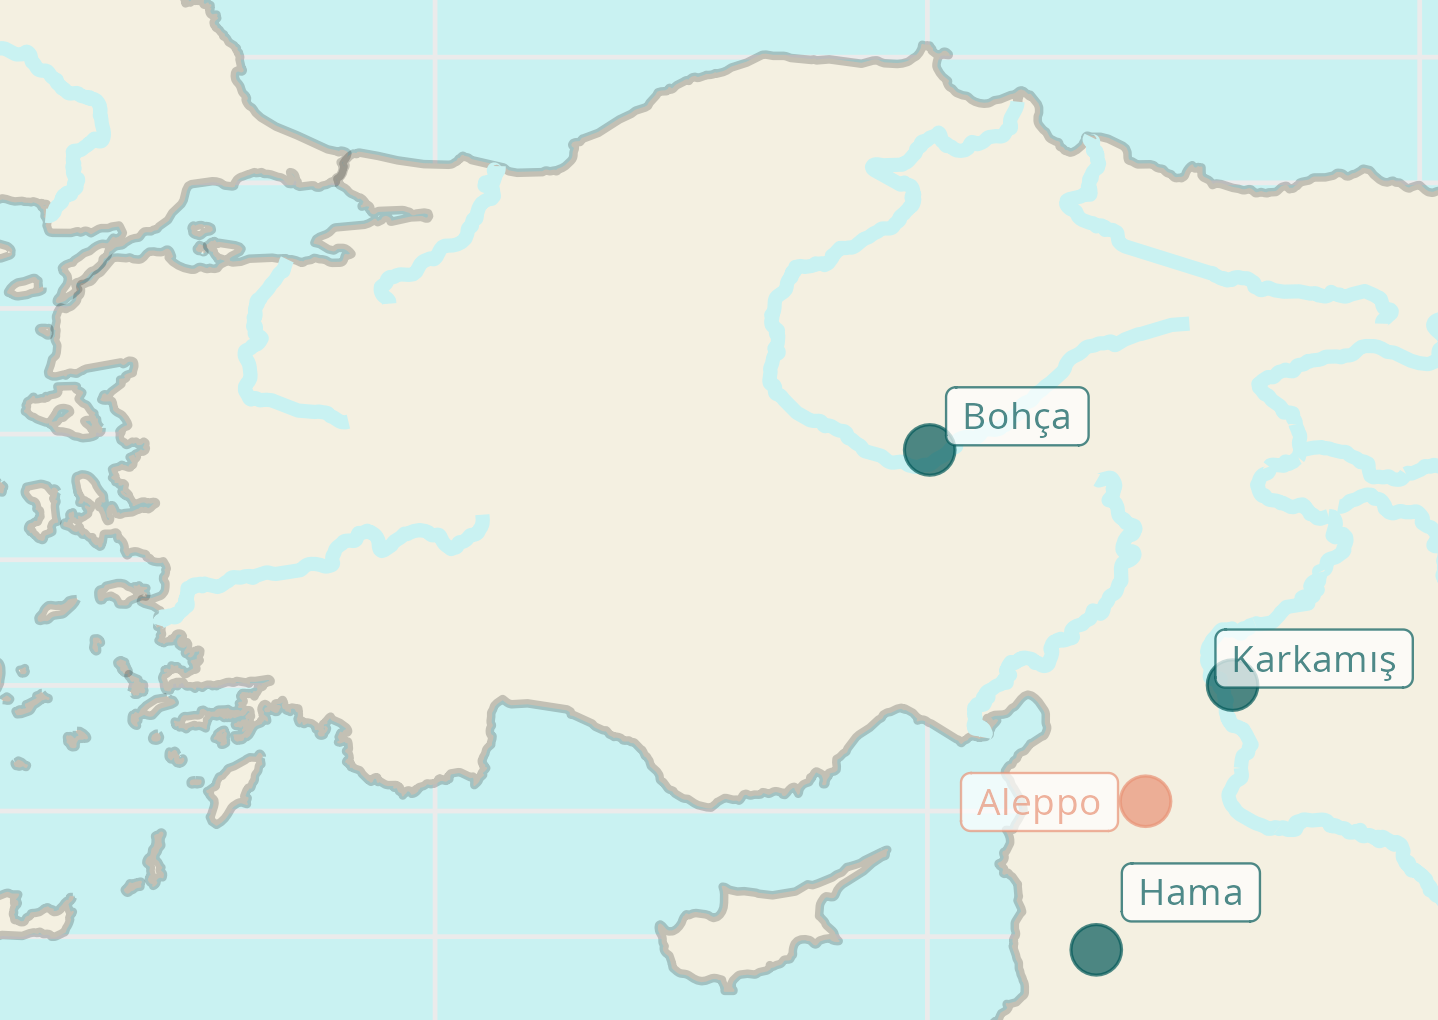
\includegraphics[width=0.8\textwidth]{../../../Mídia/Map04.png}
\end{center}

\clearpage

Karkamiš teria sido uma cidade fortificada por duas camadas de muralhas, o
centro administrativo estando na esfera mais interna, com acesso direto ao rio
Eufrates ao nordeste.
Dentro deste círculo, entende-se que a cidade teria dois complexos palaciais, um
na cidade baixa e o outro na cidade alta.
A parte mais bem escavada é o complexo palaciano inferior, com
construções identificadas desde o portão ao lado do rio Eufrates até o portão
real que levaria à cidade alta.

\begin{figure}[h!]
	\begin{center}
		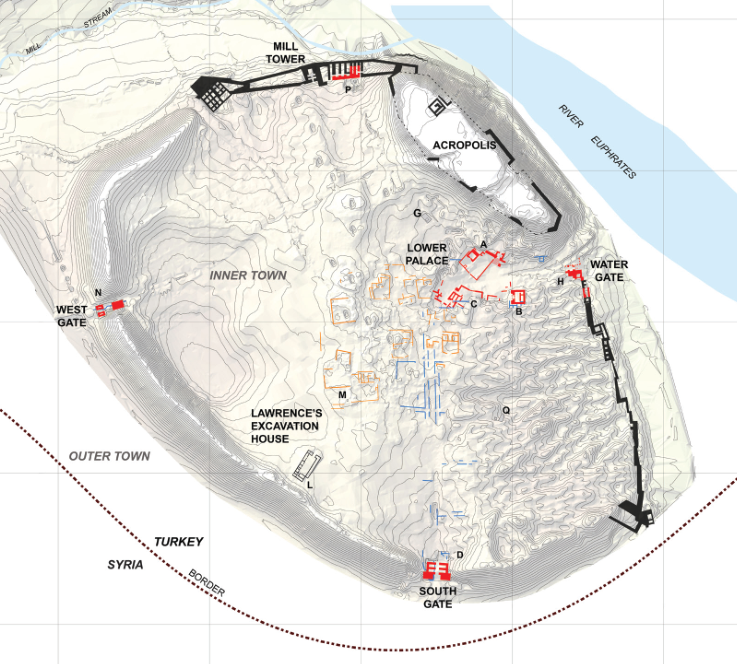
\includegraphics[width=0.8\textwidth]{../../../Mídia/karkemis00.png}
	\end{center}
	\begin{center}
		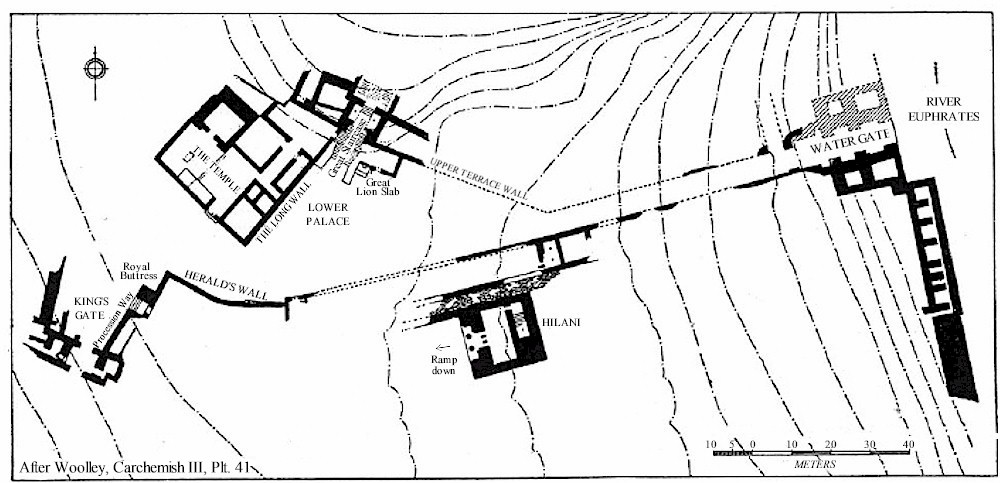
\includegraphics[width=\textwidth]{../../../Mídia/kargamis01.jpg}
	\end{center}
	\caption[Mapas de Karkamiš]{Mapas de Karkamiš~\cite[22]{Marchetti2014} e do
		complexo palaciano inferior~\cite[\emph{plate} 41]{CarchemishIII}.}\label{fig:mapa-kark1}
\end{figure}

A maior parte das inscrições provém de ortostatos (blocos de pedra verticais
utilizados na construção de um muro), incluindo KARKAMIŠ A11\emph{b}+\emph{c} (=
A9 e 10).
Escavados nas operações de 1911--14, as peças tinham sido reutilizadas como
pavimento, com o texto virado para baixo,
no umbral do ``Portão do Rei'', próximas da inscrição A11\emph{a},
encontrada \emph{in situ} (\autoref{fig:portao-real}).

\begin{figure}[h!]
	\begin{center}
		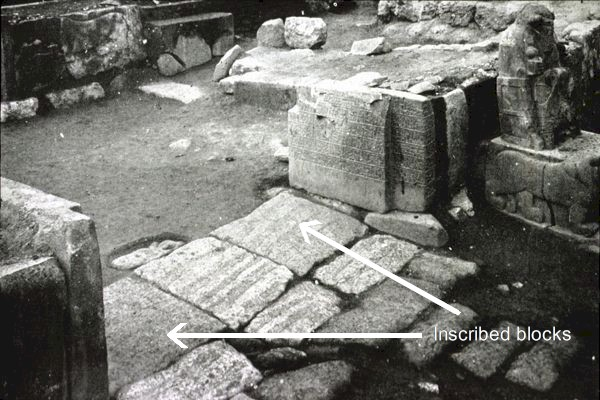
\includegraphics[width=0.95\textwidth]{../../../Mídia/kargamis08.jpg}
		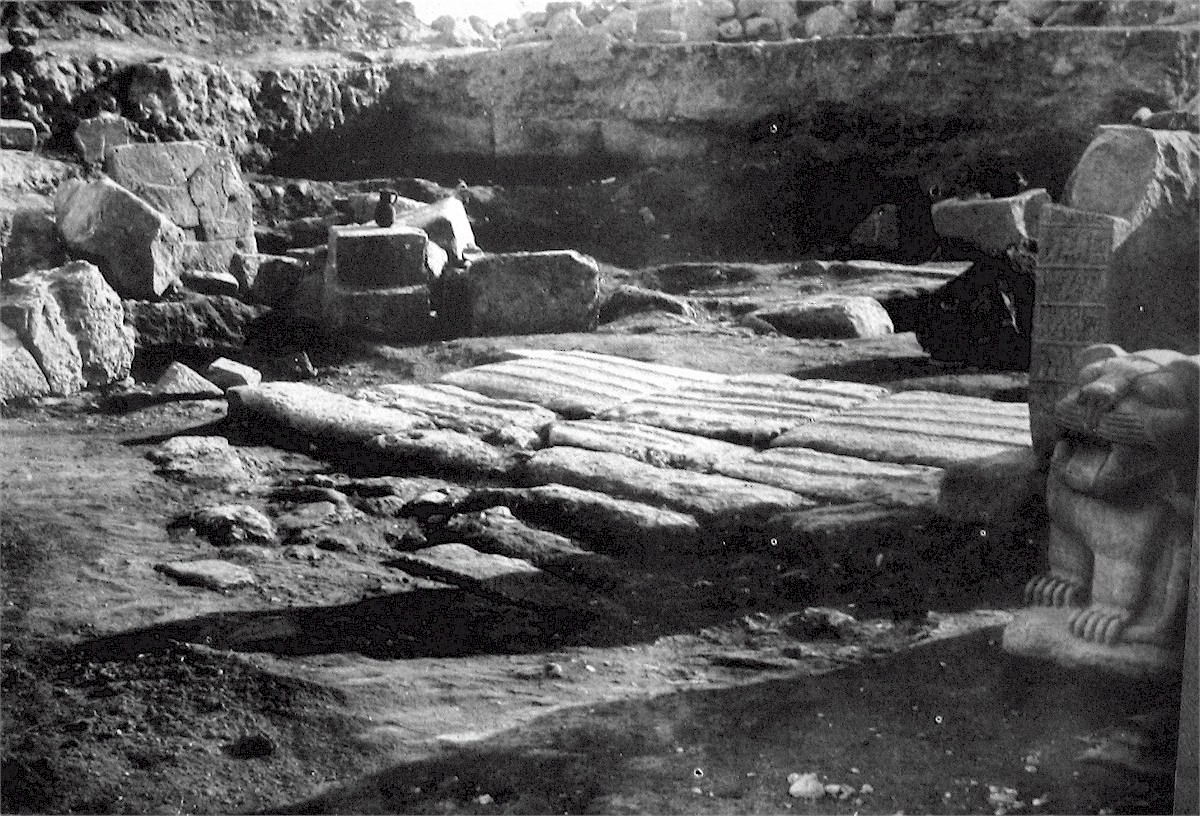
\includegraphics[width=0.95\textwidth]{../../../Mídia/kargamis111.jpg}
	\end{center}
	\caption[``Portão do Rei'' em Karkamiš]{Portão do Rei em Karkamiš. Em pé
		vê-se a inscrição A11\emph{a} e o pavimento imediatamente ao lado é
		composto pelos ortostatos da inscrição A11\emph{b}+\emph{c}. Imagens
		de~\cite[\emph{plates} 46--7]{CarchemishIII}.}\label{fig:portao-real}
\end{figure}



O conteúdo do texto de KARKAMIŠ A11\emph{b}+\emph{c} e o material utilizado
fazem supor que os dois ortostatos utilizados na inscrição faziam parte do
``Contraforte Real'', antes do ``Caminho de Procissão'', alguns metros antes do
``Portão do Rei'' (ver~\autoref{fig:mapa-kark1}) e
as peça A11\emph{b} (= A9) e A11\emph{c} (= A10) devem ter sido parte de batentes
de uma porta \slash{} portão, dispostas do lado direito e esquerdo,
respectivamente.
As peças narram o que parece ter sido uma revolta na cidade protagonizada por
figuras mencionadas por \emph{netos de Uratarhunta}; a reconquista da cidade
simultaneamente à conquista de Kawa com apoio dos deuses; a construção dos
andares superiores do ``Caminho de Procissão'' e o estabelecimento de culto às
divindades Tarhunta, Karhuha, Kubaba e Sarku.
Em meio ao texto, estabelece-se os sacrifícios estipulados às divindades,
maldições de proteção e uma justificativa para a construção dos andares
superiores, talvez indicando que o uso deste espaço seria voltado a mulheres de
alguma forma.
Os ortostatos hoje estão no Anadolu Medeniyetleri Müzesi em Ankara.

\begin{figure}[h]
	\centering
	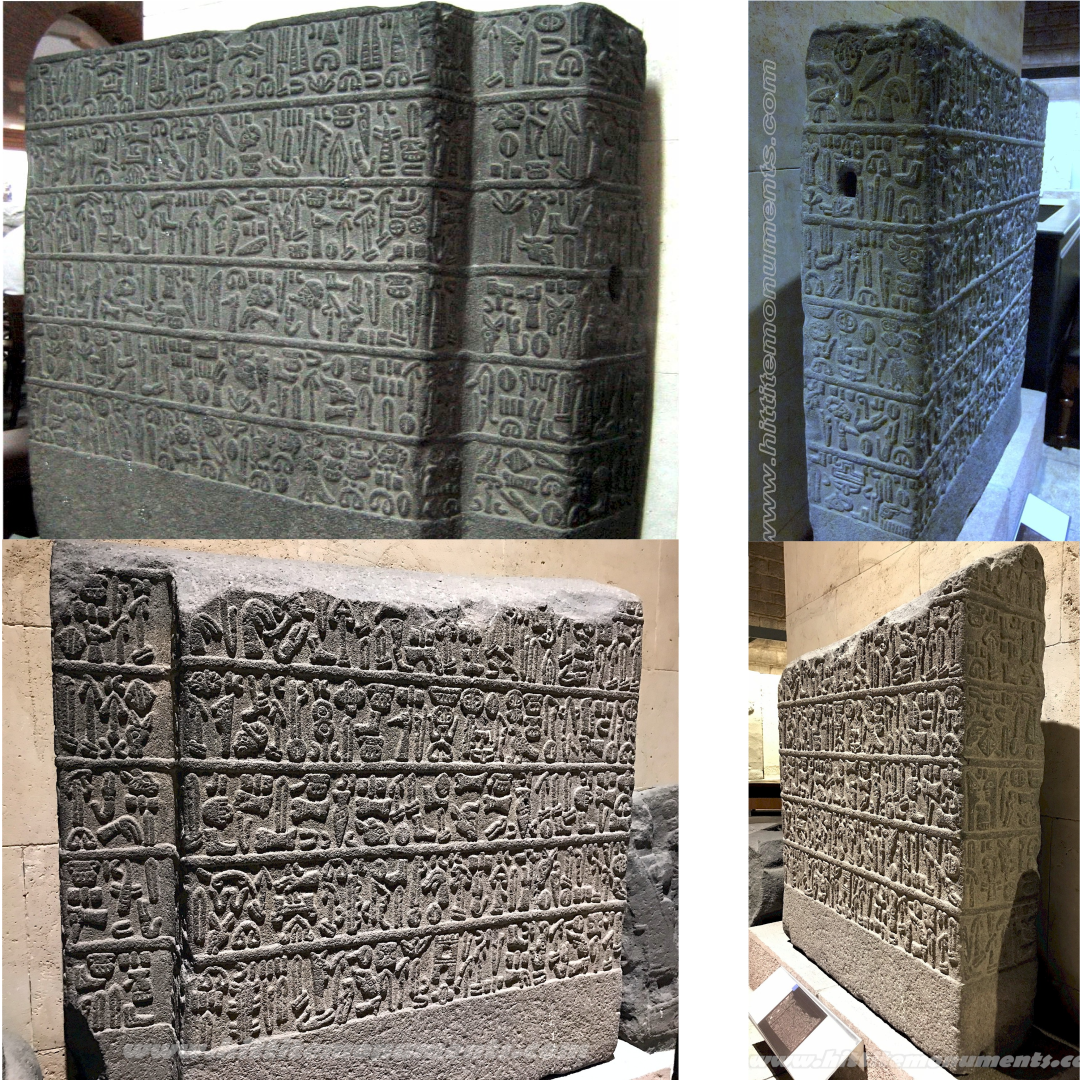
\includegraphics[width=0.9\textwidth]{../../../Mídia/karkamisA11bc.png}

	\caption[KARKAMIŠ A11\emph{b}+\emph{c}]{Inscrição KARKAMIŠ A11\emph{b}+\emph{c}.
		Dimensões da inscrição:
		\emph{b} 0.83\times1.60\times0.23m,
		\emph{c} 0.86\times1.55\times0.23m.
		Imagens de Tayfun Bilgin, 2006,
		disponíveis em
		\href{https://www.hittitemonuments.com/karkamis/kargamis43.htm}{Hittite Monuments}.
		Edição e traçado em~\citeabbrev*{CHLI11}, pp.\ 101ff.\ e \emph{plate}
		14--17.
	}\label{fig:karkamisA11b}
\end{figure}

\begin{center}
	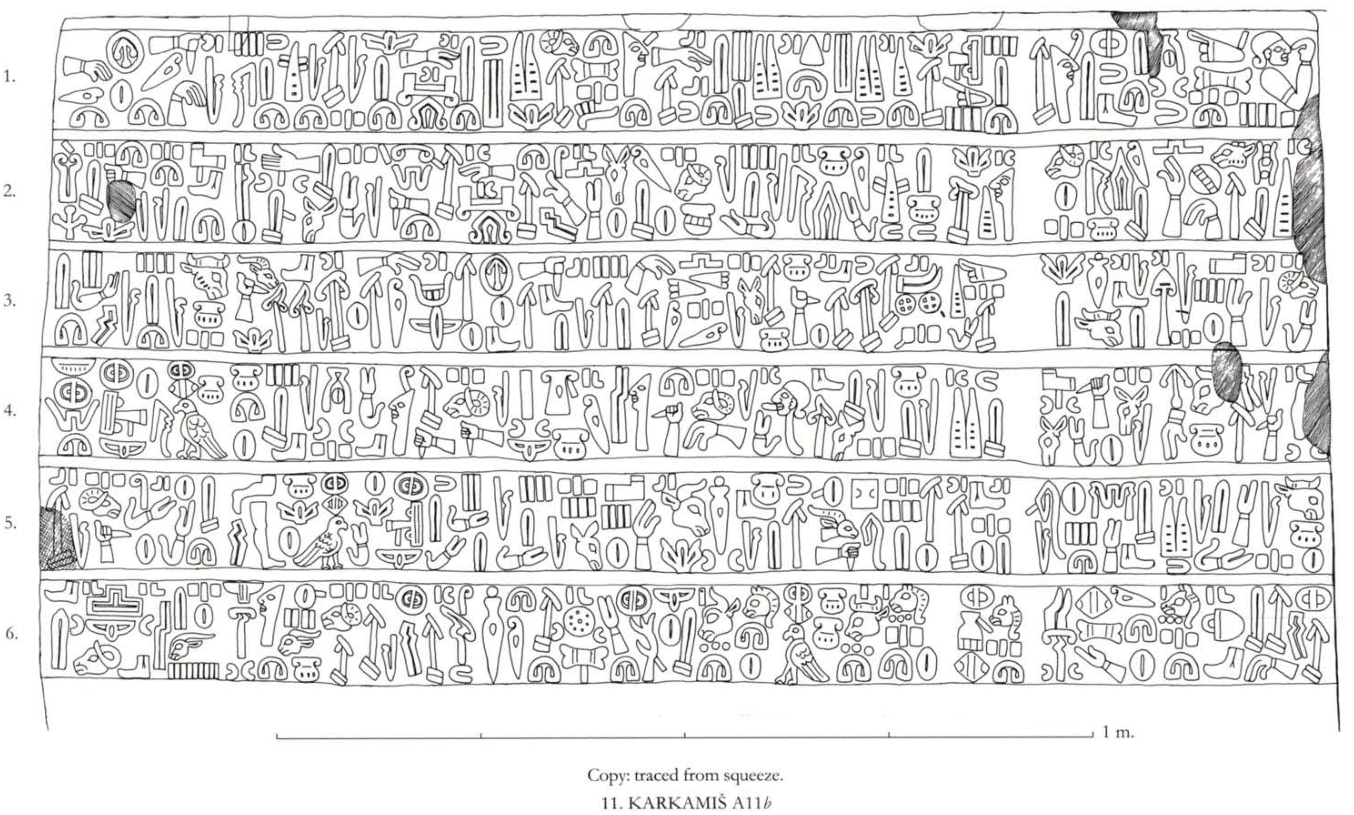
\includegraphics[height=\textwidth, angle=90]{../../../Mídia/karkamisA11b.png}
\end{center}

\clearpage

\begin{center}
	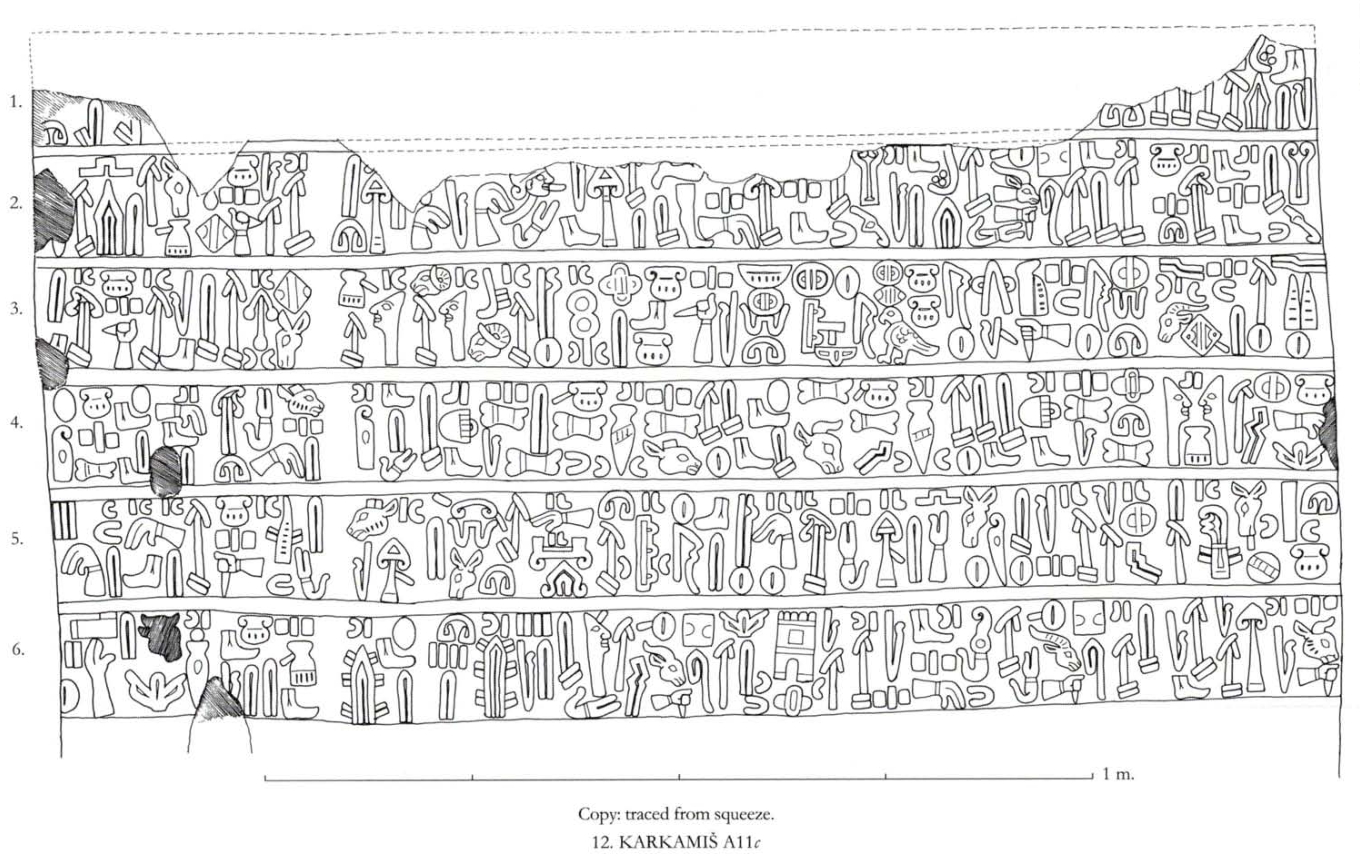
\includegraphics[height=\textwidth, angle=90]{../../../Mídia/karkamisA11c.png}
\end{center}

\clearpage

\setcounter{parcount}{0}
\begin{parnumbersa}[]

	\raggedright%
	\itshape%

	\logo{EGO}-wa/i-mi \spac{}ka-tú-wa/i-sa \logo{“IUSTITIA”}-ni-i-sa
	\logo{DEUS}-ni-ti-i \logo{(LITUUS)}á-za-mi-i-sa
	kar-ka-mi-si-za-sa\logo{(URBS)} \lmasc{}\logo{REGIO}-ni \logo{DOMINUS}-sa
	\spac{}su-hi-si \lmasc{}\logo{REGIO}-ni \logo{DOMINUS}-ia-i-sa
	\lmasc{}\logo{FILIUS.}NI-za-sa \spac{}á-sa-tú-wa/i-lá/í-ma-za-si \logo{REGIO}-ni \logo{DOMINUS}-i-sa \lmasc{}\logo{FILIUS.NEPOS}-si-i-sa

	a-wa/i za-a-sa \logo{URBS+}MI-ni-i-sa mi-sá-*a \lmasc{}tá-da-li-sa
	\logo{AVUS}-ha-da-li-sa \lbreak{} \spac{}\logo{*447}-nu-wa/i-ia-si sa-tá-*a

	wa/i-sa-*a \logo{VACUUS}-ti-i-sa \lmasc{}\logo{ARHA} \logo{(“LONGUS”)}ia\logo{+} ra/i-ia-ta

	wa/i-na-*a \spac{}\logo{MAGNUS+}ra/i-\logo{TONITRUS}-tá-sa-za \lmasc{}\logo{FILIUS.NEPOS}-sa-za \logo{CUM}-ní \lmasc{}\logo{(LOCUS)}pi-ta-ha-li-ia-ha

	wa/i-ma-zá-*a mi-i-na-*a \lmasc{}sá-pa-la/i-li-na \lmasc{}\logo{URBS+}MI-ni i-pa-ni-si-ná\logo{(URBS)} \lmasc{}á-ma-ha-wa/i \lmasc{}sá-pa-lá/í-li-ia \logo{TERRA.PONERE}-ru-da mu-zi-ki-ia\logo{(URBS)} \lmasc{}$[$\logo{\ldots{}}$]$ \lbreak{}

	wa/i-ma-na-a* \lmasc{}\logo{AEDIFICARE}-\logo{MI}-ha

	a-wa/i \lmasc{}\logo{REL}-a-ti-i \lmasc{}\logo{(ANNUS)}u-si-i
	ka-wa/i-za-na\logo{(URBS)} \lmasc{}\logo{(CURRUS)}wa/i\logo{+}ra/i-za-ni-ná
	\lmasc{}\logo{PES\textsubscript{2}}-za-ha

	pa-tá-za-pa-wa/i-ta-*a \logo{(TERRA+LA+LA)}wa/i-li-li-da-za mi-i-zi-*a
	\lmasc{}tá-ti-i-zi \logo{AVUS}-ha-ti-zi-ha
	\lmasc{}\logo{*348}{(-)}lu/a/i\textsuperscript{?}-da-li-zi-ha
	\lmasc{}\logo{NEG\textsubscript{2}}-a \logo{(PES\textsubscript{2})}hwi/a-hwi/a-sà-tá-si


\end{parnumbersa}

\vspace{10pt}
\hrule
\vspace{10pt}


\setcounter{parcount}{0}
\begin{parnumbersa}[]

	\raggedright%
	\itshape%

	amu=wa=mi Katuwas, tarawanis, masanidi azamis, Karkamisizas
	\logo{REGIO}-ni-\logo{DOMINUS}-s,
	Suhisi \logo{REGIO}-ni-\logo{DOMINUS}-yais nimuwizas,
	Asatuwalamanzasi \logo{REGIO}-ni-\logo{DOMINUS}-is hamsis.

	a=wa zas \logo{URBS+}MI-nis tadallis huhadallis Ninuwis asta.

	a=wa=as tanatis arha yariyata.

	a=wa=an Uratarhuntasanza hamsanza \logo{CUM}-ni pitahaliyaha.

	a=wa=manza amin sapalalin \logo{URBS+}MI-nin Ipanisin, ama=ha=wa sapalaliya
	\logo{TERRA.PONERE}-ruda Muzikiya \ldots{}

	a=wa=mw=an tamaha.

	a=wa kwati usi Kawazan warazanin wazaha,


	apatanza=pa=wa=ta walilidanza aminzi tatinzi huhatinzi=ha \logo{*348}-dalinzi=ha na hwihwisantasi


\end{parnumbersa}

\vspace{10pt}
\hrule
\vspace{10pt}

[1] Eu sou Katuwa, justo, amado pelos deuses, senhor regional de Karkamis, filho
de Suhis, o senhor regional, neto de Asatuwalamaza, o senhor regional.
	[2] Esta cidade do meu pai e avô era\slash{}tornou-se (de?) Ninuwi,
[3] E ela esticou-se em vão {???.}
[4] E com os netos de Uratarhunta eu PITAHALIYA-ei,
[5] E para eles minha cidade SAPALALI Ipanis e minhas SAPALALI-s {???} Muzikis {???}.
[6] Eu mesmo a construí,
[7] no ano em que eu movi a campanha pela cidade de Kawaza,
[8] para aqueles territórios meus pais, avós, bisavós não marcharam.

\clearpage

\setcounter{parcount}{8}
\begin{parnumbersa}[]

	\raggedright%
	\itshape%

	mu-pa-wa/i-*a mi-i-sa-*a \logo{(DOMINUS)}na-ní-i-sa \lbreak{} \logo{CAELUM} \logo{(DEUS)}\logo{TONITRUS}-sa \logo{(DEUS)}kar-hu-ha-sá \logo{(DEUS)}ku\logo{+AVIS}-pa-pa-sa-ha mi-ia-ti-*a \logo{“IUSTITIA”}-wa/i-na-ti \logo{(LITUUS)}á-za-tá

	wa/i-ma-tá-*a \logo{(“LIGNUM”)}hu-hú\logo{+}ra/i-pa-li \lmasc{}\logo{(SOLIUM)}á-sa-tá

	wa/i-ma-da-*a \lmasc{}\logo{PRAE}-na \logo{(PES\textsubscript2)}hwi/a-ia-ta

	a-wa/i pa-ia-*a \lmasc{}\logo{REGIO}-ni-ia \logo{(“VACUUS”)}ta-na-tá-ha

	wa/i-ta-*a \logo{(SCALPRUM.CAPERE2)}u-pa-ní-zi a-tá \lmasc{}\logo{(“CAPERE2”)}\lbreak{}u-pa-ha

	a-wa/i pi-i-na-*a \lmasc{}\logo{REGIO}-ni-ia-ti \logo{(FULGUR)}pi-ha-mi-sa \logo{SUPER+}ra/i-a \lmasc{}\logo{PES}-wa/i-i-ha

	\lmasc{}za-zi-ha-wa/i-mi-i \logo{(DOMUS.SUPER)}ha\logo{+}ra/i-sà-tá-ni-zi pa-ti-i-*a \logo{(“ANNUS”)}u-si \lmasc{}\logo{AEDIFICARE}-\logo{MI}-ha


\end{parnumbersa}

\vspace{10pt}
\hrule
\vspace{10pt}


\setcounter{parcount}{8}
\begin{parnumbersa}[]

	\raggedright%
	\itshape%

	amu=pa=wa nanis tipasis Tarhuntas, Karhuhas, Kubabas=ha amiyati tarwanadi
	azanta.

	a=wa=mw=a\emph{t}a huhurpali asanta,

	a=wa=mw=ada paran hwiyanta.

	a=wa apaya \logo{REGIO}-niya tanataha.

	a=wa=ta upaninzi anta upaha.

	a=wa apin \logo{REGIO}-niyadi pihamis sara awiha.

	zanzi=ha=wa=mi haristaninzi apati usi tamaha.



\end{parnumbersa}

\vspace{10pt}
\hrule
\vspace{10pt}


[9] Mas a mim o senhor celeste Tarhunta, Karhuha e Kubaba pela minha justiça
amavam,
[10] eles me sentaram no HUHURPALA,
[11] eles correram na minha frente
	[12] e eu destruí aquelas regiões.

[13] Eu trouxe prêmios para dentro,
[14] eu voltei glorioso daquelas regiões,
[15] e estes andares superiores eu construí naquele ano.


\clearpage

\setcounter{parcount}{15}
\begin{parnumbersa}[]

	\raggedright%
	\itshape%


	wa/i-mi-ta-*a mi-i-na-*a \logo{(DOMINUS)}na-<<i>>-ni-i-na \logo{(DEUS)}kar-hu-ha-si-na \logo{(DEUS)}ku\logo{+AVIS}-pa-si-ha \logo{CRUS2}\logo{.CRUS}{(-)}ní-ia-sa-ha-na \lmasc{}\logo{LITUUS+}na-ha

	wa/i-ma-tá-*a \lmasc{}za\lbreak{}-ti-i \lmasc{}\logo{(“PODIUM”)}hu-ma-ti \lmasc{}\logo{(SOLIUM)}i-sà-nú-wa/i-ha

	\logo{(“*350”)}á-sa-ha\logo{+}ra/i-mi-sà-pa-wa/i-ma-za \lmasc{}za-a \logo{DEUS}-ní-za
	\lmasc{}\logo{CUM}-ni \logo{ANNUS}-sa-li-za-sa
	\lmasc{}\logo{(“PANIS”)}tú\logo{+}ra/i-pi-sa
	\logo{(DEUS)}\logo{CERVUS\textsubscript{3}+}ra/i-hu-ha-ia 1
	\logo{BOS}\logo{(ANIMA)}-sa \logo{OVIS}-sa-ha
	\logo{(DEUS)}ku\logo{+AVIS}-pa-pa 1 \logo{BOS}\logo{(ANIMA)}-sa 1
	\logo{OVIS}\logo{(ANIMA)}-wa/i-sa-ha
	\logo{(DEUS)}sa\textsubscript{5}\logo{+}ra/i-ku \logo{OVIS}-wa/i-sa \logo{(“*478”)}ku-tú-pi-li-sa-ha 1 \logo{OVIS}\logo{(ANIMA)}-wa/i-sa \lmasc{}\logo{VIR}-ti-ia-da-za \logo{DEUS}-ní-za \lbreak{} $[$1 \logo{OVIS}\logo{(ANIMA)}-wa/i$]$-sa $[$\logo{FEMINA}-ti$]$-ia-$[$ta$]$-za $[$\logo{DEUS}-ni-za$]$


\end{parnumbersa}

\vspace{10pt}
\hrule
\vspace{10pt}


\setcounter{parcount}{15}
\begin{parnumbersa}[]

	\raggedright%
	\itshape%


	a=wa=mi=ta amin nanin Karhuhasin Kubabasin=ha niyashan \logo{LITUUS}+naha.

	a=wa=mw=ata zati humati isanuwaha.

	asharimis=pa=wa=manza za masani{(ya)}nza \logo{CUM}-ni usalizas turpis:
	Karhuhaya 1 wawis hawas=ha;
	Kubaba 1 wawis hawas=ha;
	Sarku hawas kutupilis=ha;
	1 hawas zidiyadanza masani{(ya)}nza; $[$1 hawa$]$s $[$wanati$]$ya$[$ta$]$nza
	masani{(ya)}nza.


\end{parnumbersa}

\vspace{10pt}
\hrule
\vspace{10pt}


[16] E eu vi pessoalmente a procissão do meu senhor Karhuha e Kubaba,
[17] e eu mesmo os sentei neste altar.
	[18] O sacrifício de sangue para estes (seja):
para os deuses em conjunto, o pão anual;
para Karhuha, 1 touro e uma ovelha;
(para) Kubaba, 1 touro e uma ovelha;
(para) Sarku, uma ovelha e um KUTUPILI\@;
1 ovelha para os deuses masculinos;
1 ovelha para as deusas femininas.

\clearpage

\setcounter{parcount}{18}
\begin{parnumbersa}[]

	\raggedright%
	\itshape%


	$[$\logo{\ldots{}}$]$-sa z$[$a-ti$]$-ia-za $[$\logo{DEUS}-n$]$i\textsuperscript{?}-za \logo{MALUS}-la/i-ti-i-*a \lbreak{} \logo{VERSUS}-ia-ni \lmasc{}\logo{PES}-wa/i-ti

	\lmasc{}\logo{NEG\textsubscript{2}}-pa-wa/i-sa \lmasc{}za-ti-ia-za \logo{(DOMUS.SUPER)}ha\logo{+}ra/i-sà-tá-na-za \logo{MALUS}-la/i-ti-i-*a \lmasc{}\logo{VERSUS}-ia-ni $[$\logo{PES}$]$-wa/i-ti

	$[$\lmasc{}$]$\logo{NEG\textsubscript{2}}-$[$pa$]$-wa/i-da
	\logo{CRUS2.CRUS}$[${(-)}ni\textsuperscript{?}$]$-ia-za-i \logo{REL}-a-ti \logo{PRAE}-na

	$[$wa/i$]$-da-*a $[$\logo{SCRIBA+RA/I}$]$\logo{CAPERE}/da-\textsc{⌈}i\textsc{⌉} \textsc{⌈}\lmasc{}\textsc{⌉}\logo{REL}-i-sa

	\lmasc{}za-a-zi-pa-wa/i-tá
	$[$\logo{(SCALPRUM)}$]$ku-ta-sa\textsubscript{5}\logo{+}ra/i-zi-i
	\logo{LOCUS}-la/i-za-\textsc{⌈}*a\textsc{⌉} [\textsuperscript{?}]\lbreak{}-i-t[i]

	\lmasc{}\logo{NEG\textsubscript{2}}-pa-wa/i-tá \lmasc{}za-a-ti-ia-za
	\lmasc{}\logo{(“SCALPRUM”)}ku-ta-sa\textsubscript{5}\logo{+}ra/i-za \lmasc{}á-ma-za \lmasc{}á-lá/í-ma-za \lmasc{}\logo{ARHA} \lmasc{}\logo{“MALLEUS”}-lu/a/i-i

	pa-ti-pa-wa/i-tá-*a \logo{CAELUM} \logo{(DEUS)}\logo{TONITRUS}-sa \logo{(DEUS)}kar-hu-ha-sá \logo{(DEUS)}ku\logo{+AVIS}-pa-pa-sá-ha \logo{(MONS)}a\logo{+}ra/i-pu-tá-wa/i-ni-sá-ha \logo{(DEUS)}\logo{TONITRUS}-sa \logo{(“FLUMEN+MINUS”)}sà-ku\logo{+}ra/i-wa/i-ni-i-zi-ha \logo{(FLUMEN.REGIO)}ha\lbreak{}-pa-da-si \logo{DEUS}-ní-zi \lmasc{}\logo{LIS}-lu/a/i-sa-tú

	wa/i-tú-*a \lmasc{}\logo{VIR}-ti-ia-ti-ia-za-ha \lmasc{}\logo{(“CULTER”)}pa\logo{+}ra/i-tú-ní-tú-u

	\logo{FEMINA}-ti-ia-ti-ia-za-ha-wa/i-tú-u \lmasc{}\logo{(“CULTER”)}pa\logo{+}ra/i-tú-ni-i-tú

	wa/i-tú-*a \lmasc{}\logo{VIR}-ti-ia-ti-i-na \lmasc{}\logo{(*462)}mu-wa/i-i-da-na \logo{NEG3}-sa \lmasc{}\logo{CAPERE}-ti-i

	\logo{FEMINA}-ti-i$[$a$]$-ti-pa-wa/i-tú
	\logo{(FEMINA.*462)}\lbreak{}{4}\textsuperscript{?}-da \lmasc{}ni-i \lmasc{}\logo{CAPERE}-ti-i


\end{parnumbersa}

\vspace{10pt}
\hrule
\vspace{10pt}


\setcounter{parcount}{18}
\begin{parnumbersa}[]

	\raggedright%
	\itshape%



	$[$kwis$]$-s za$[$ti$]$yanza $[$masani$]${(ya)}nza atuwalidi
	tawiyan awati,

	napa=wa=as zatiyanza haristananza atuwalidi tawiyan $[$a$]$wati,

	na$[$pa$]$=wa=ada $[$ni$]$yazai kwati paran,

	a=$[$wa$]$=ada \logo{SCRIBA+}ra-\logo{CAPARE}dai kwis,

	zanzi=pa=wa=ta kutasarinzi arlanza {?}-iti

	napa=wa=ta zatiyanza kutasari{(ya)}nza amanza alamanza arha walai,

	apati=pa=wa=ta tipasis Tarhuntas, Karhuhas, Kubabas=ha, arputawanis=ha
	Tarhuntas, Sakurawaninzi=ha hapadasi masaninzi \logo{LIS}-lu/a/i-santu.

	a=wa=tu zidiyadiya=za partunintu,

	wanatiyatiya=za=ha=wa=tu partunintu.

	a=wa=tu zidiyadin muwidan nis lanti,

	wanatiyatin=pa=wa=tu muwidan ni lanti.

\end{parnumbersa}

\vspace{10pt}
\hrule
\vspace{10pt}



\ldots{}
[19] Aquele que se aproximar destes deuses com maldade,
[20] ou que se aproximar desses andares superiores com maldade,
[21] ou se eles seguirem {?}para baixo / {?}transferirem a alguém,
[22] que {???}
	[23] e que {???} estes murais do seus lugares,
[24] ou apague meu nome desses murais,
[25] contra ele o celeste Tarhuta, Karhuha, Kubaba, Tarhunta do Monte Arputa e
os deuses da terra fluvial do rio Sakura litiguem!
[26] Que dele arranquem a masculinidade,
[27] que dela arranquem a feminilidade,
[28] que dele eles não tomem a semente masculina,
[29] que dela eles não tomem a semente feminina.

\clearpage

\setcounter{parcount}{29}
\begin{parnumbersa}[]

	\raggedright%
	\itshape%


	\lmasc{}za-pa-wa/i-tá \lmasc{}\logo{URBS+}MI-ni-i-na mu-*a
	\lmasc{}\logo{REL+}ra/i-i \spac{}\logo{MAGNUS+}ra/i-\logo{TONITRUS}-ta-sa-za
	\lmasc{}\logo{FILIUS.NEPOS}-sa-za \lmasc{}\logo{(“*314”)}ha-sá-ti-i \logo{ARHA} \lmasc{}\logo{CAPERE}-ha

	\lmasc{}\logo{NEG\textsubscript{2}}-wa/i-na \lmasc{}\logo{REL+}ra/i-i \logo{(LOCUS)}pi-ta-ha-li-ia-ha

	a-wa/i \lmasc{}za-a-zi \lmasc{}\logo{DEUS}-ní-i-zi \lmasc{}\logo{AUDIRE+MI}-ta\logo{+}ra/i-ru

	\logo{“LIGNUM”}-sa-pa\lbreak{}-wa/i-mu-tá-a \lmasc{}\logo{REL}-a-za za-a-ti-ia-za \lmasc{}\logo{(DOMUS.SUPER)}ha\logo{+}ra/i-sà-tá-na-za \logo{POST}-ni \lmasc{}\logo{PES}-wa/i-da

	a-wa/i \lmasc{}za-a-zi \logo{“PORTA”}-lu/a/i-ni-si-i-zi
	\logo{(DOMUS.SUPER)}ha\logo{+}ra/i-sà-tá-ní-zi \spac{}á-na-ia mi-i-*a
	\lmasc{}\logo{BONUS}-sa-mi-i \logo{FEMINA}-ti-i
	\lmasc{}\logo{(BONUS)}wa/i-sa\textsubscript{5}\logo{+}ra/i-ti-i pa-ti-i-*a \lmasc{}\logo{(ANNUS)}u-si-i \logo{AEDIFICARE}-\logo{MI}-h$[$a$]$


\end{parnumbersa}

\vspace{10pt}
\hrule
\vspace{10pt}


\setcounter{parcount}{29}
\begin{parnumbersa}[]

	\raggedright%
	\itshape%


	zan=pa=wa=ta \logo{URBS+}MI-nin amu kwari Uratarhuntasanza hamsanza hasadi arha laha

	na=wa=an kwari pitahaliyaha,

	a=wa zanzi masaninzi tumantintaru.

	taruwis=wa=mu=ta kwanza zatiyanza haristananza apan awada,

	a=wa zanzi \logo{PORTA}-lanisinzi haristanninzi Anaya ami wasami wanati wasaradi
	apati usi tamaha.


\end{parnumbersa}

\vspace{10pt}
\hrule
\vspace{10pt}


[30] Se eu mesmo tomei esta cidade dos netos de Uratarhunta à força,
[31] e se ela eu não PITAHALIYA-ei,
[32] sejam estes deuses testemunhas.

	[33] Porque a madeira para estes andares superiores chegou depois para mim,
[34] estes andares superiores dos portais à Ana, minha boa mulher, com bondade
construí naquele ano.

\clearpage
\begin{multicols}{2}[\noindent\textbf{Vocabulário}]
	\begin{hangparas}{1em}{1}
		\raggedright%
		\textbf{\emph{\emph{*348}-dali-}} (\emph{subst.com.}) \tabto{1em} bisavô?\\
		\textbf{\emph{alamanza-}} (\emph{subst.neut.}) \tabto{1em} nome\\
		\textbf{\emph{Ana-}} (\emph{NP}) \tabto{1em} Ana\\
		\textbf{\emph{arla-}} (\emph{subst.neut.}) \tabto{1em} lugar\\
		\textbf{\emph{Arputawani-}} (\emph{adj.}) \tabto{1em} relacionado ao monte Arputa\\
		\textbf{\emph{Asatuwalamanza-}} (\emph{NP}) \tabto{1em} Asatuwalamanza\\
		\textbf{\emph{asharimi{(s)}-}} (\emph{subst.neut.}) \tabto{1em} sacrifício (de sangue)\\
		\textbf{\emph{atuwal{(i)}-}} (\emph{adj.}) \tabto{1em} mau\\
		\textbf{\emph{awa-}} (\emph{v.i.}) \tabto{1em} ir, ir fazer\\
		\textbf{\emph{aza-}} (\emph{v.t.}) \tabto{1em} amar\\
		\textbf{\emph{\emph{CUM}-ni}} (\emph{prep.}) \tabto{1em} com\\
		\textbf{\emph{hamsi}} (\emph{subst.com.}) \tabto{1em} neto\\
		\textbf{\emph{hapadi-}} (\emph{adj.}) \tabto{1em} fluvial\\
		\textbf{\emph{haristani-}} (\emph{subst.}) \tabto{1em} andar superior  aposento?\\
		\textbf{\emph{hasa-}} (\emph{subst.neut.}) \tabto{1em} força\\
		\textbf{\emph{hawa-}} (\emph{subst.com.}) \tabto{1em} ovelha\\
		\textbf{\emph{huha-}} (\emph{subst.com.}) \tabto{1em} avô\\
		\textbf{\emph{huhadall{(a/i)}-}} (\emph{adj.}) \tabto{1em} ancestral\\
		\textbf{\emph{huhurpali-}} (\emph{subst.neut.}) \tabto{1em} {?}, algo feito de madeira\\
		\textbf{\emph{humati-}} (\emph{subst.}) \tabto{1em} pódium, altar (de madeira)\\
		\textbf{\emph{hwihwisa-}} (\emph{v.i.}) \tabto{1em} correr (iterativo de \emph{hwi{(ya)}-})\\
		\textbf{\emph{hwi{(ya)}-}} (\emph{v.i.}) \tabto{1em} correr\\
		\textbf{\emph{Ipanisi-}} (\emph{TO}) \tabto{1em} Ipanisi\\
		\textbf{\emph{isanuwa-}} (\emph{v.t.}) \tabto{1em} fazer sentar (causativo de \emph{asa-})\\
		\textbf{\emph{Karhuha-}} (\emph{TE}) \tabto{1em} Karhuha\\
		\textbf{\emph{Karhuhasa-}} (\emph{adj.poss.}) \tabto{1em} de Karhuha\\
		\textbf{\emph{Karkamisiza-}} (\emph{adj.}) \tabto{1em} de Karkamiš\\
		\textbf{\emph{Katuwa-}} (\emph{NP}) \tabto{1em} Katuwa\\
		\textbf{\emph{Kawaza-}} (\emph{TO}) \tabto{1em} Kawa\\
		\textbf{\emph{Kubaba-}} (\emph{TE}) \tabto{1em} Kubaba\\
		\textbf{\emph{Kubabasa-}} (\emph{adj.poss.}) \tabto{1em} Kubaba\\
		\textbf{\emph{kutasari-}} (\emph{subst.neut.}) \tabto{1em} ortostato, mural\\
		\textbf{\emph{kutupili-}} (\emph{subst.com.}) \tabto{1em} ovelha sacrificial?\\
		\textbf{\emph{la-}} (\emph{v.t.}) \tabto{1em} pegar\\
		\textbf{\emph{\emph{LIS}-lu/a/i-sa-}} (\emph{v.t.}) \tabto{1em} litigar contra?\\
		\textbf{\emph{\emph{LITUUS}+na-}} (\emph{v.t.}) \tabto{1em} ver\\
		\textbf{\emph{masani-}} (\emph{subst.com.}) \tabto{1em} deus, divindade\\
		\textbf{\emph{muwida-}} (\emph{subst.neut.}) \tabto{1em} semente\\
		\textbf{\emph{Muziki-}} (\emph{TO}) \tabto{1em} Muziki\\
		\textbf{\emph{nani-}} (\emph{subst.com}) \tabto{1em} senhor\\
		\textbf{\emph{napa}} (\emph{conj.}) \tabto{1em} ou\\
		\textbf{\emph{nimuwiza-}} (\emph{subst.com}) \tabto{1em} filho\\
		\textbf{\emph{Ninuwi-}} (\emph{NP}) \tabto{1em} Ninuwi\\
		\textbf{\emph{niyasha-}} (\emph{subst.com.}) \tabto{1em} procissão? (ver \emph{niyaza}-/\emph{niyasa-})\\
		\textbf{\emph{niyaza-/niyasa-}} (\emph{v.t.}) \tabto{1em} seguir\\
		\textbf{\emph{partuni-}} (\emph{v.t.}) \tabto{1em} cortar?\\
		\textbf{\emph{pihami-}} (\emph{adj.}) \tabto{1em} gloriado, vitorioso\\
		\textbf{\emph{pitahaliya-}} (\emph{v.t.}) \tabto{1em} adquirir???\\
		\textbf{\emph{\emph{PORTA}-lana-}} (\emph{subst.neut.}) \tabto{1em} porta, portão\\
		\textbf{\emph{\emph{REGIO}-ni-\emph{DOMINUS}-i-}} (\emph{ subst.com.}) \tabto{1em} senhor local (= hit.\ \emph{utniyasha-}?)\\
		\textbf{\emph{\emph{REGIO}-ni-}} (\emph{subst.neut.}) \tabto{1em} terra, país  povo\\
		\textbf{\emph{Sakurawani-}} (\emph{adj.}) \tabto{1em} relacionado ao rio Sakura\\
		\textbf{\emph{sapalali-}} (\emph{adj}) \tabto{1em} {?}\\
		\textbf{\emph{Sarku-}} (\emph{TE}) \tabto{1em} Sarku\\
		\textbf{\emph{\emph{SCRIBA+}ra-\emph{CAPARE}da-}} (\emph{?}) \tabto{1em} {?}\\
		\textbf{\emph{Suhi-}} (\emph{NP}) \tabto{1em} Suhi\\
		\textbf{\emph{tama-}} (\emph{v.t.}) \tabto{1em} construir\\
		\textbf{\emph{tanata-}} (\emph{v.t.}) \tabto{1em} devastar\\
		\textbf{\emph{tanati-}} (\emph{adj.}) \tabto{1em}  vazio, devastado\\
		\textbf{\emph{tarawani-}} (\emph{adj.}) \tabto{1em} justo\\
		\textbf{\emph{Tarhunta-}} (\emph{TE}) \tabto{1em} Tarhunta\\
		\textbf{\emph{taruwi-}} (\emph{subst.neut.}) \tabto{1em} madeira\\
		\textbf{\emph{tarwana-}} (\emph{subst.}) \tabto{1em} justiça\\
		\textbf{\emph{tata-}} (\emph{subst.com.}) \tabto{1em} pai\\
		\textbf{\emph{tatall{(a/i)}-}} (\emph{adj.}) \tabto{1em} paterno\\
		\textbf{\emph{tawiyan}} (\emph{adv.}) \tabto{1em} em frente a\\
		\textbf{\emph{\emph{TERRA.PONERE}-ruda}} (\emph{?}) \tabto{1em} {?}\\
		\textbf{\emph{tipasi-}} (\emph{adj.}) \tabto{1em} celeste\\
		\textbf{\emph{tumanti-}} (\emph{v.t.}) \tabto{1em} ouvir\\
		\textbf{\emph{turpi-}} (\emph{subst.neut.}) \tabto{1em} pão\\
		\textbf{\emph{upa-}} (\emph{v.t.}) \tabto{1em} trazer\\
		\textbf{\emph{upan{(i)}-}} (\emph{subst.neut.}) \tabto{1em} troféu, prêmio\\
		\textbf{\emph{Uratarhuntasa-}} (\emph{adj.poss.}) \tabto{1em} de Uratarhunta\\
		\textbf{\emph{\emph{URBS+}MI-ni-}} (\emph{subst.com.}) \tabto{1em} cidade\\
		\textbf{\emph{usaliza-}} (\emph{adj.}) \tabto{1em} anual\\
		\textbf{\emph{usi-}} (\emph{subst.neut.}) \tabto{1em} ano\\
		\textbf{\emph{wala-}} (\emph{v.i.}) \tabto{1em} morrer\\
		\textbf{\emph{walili{(da)}-}} (\emph{subst.neut.}) \tabto{1em} território\\
		\textbf{\emph{wanati-}} (\emph{subst.com.}) \tabto{1em} mulher\\
		\textbf{\emph{wanatiya-}} (\emph{adj.}) \tabto{1em} feminino\\
		\textbf{\emph{wanatiyati-}} (\emph{adj./subst.}) \tabto{1em} feminino/fêmea\\
		\textbf{\emph{wanatiyatiya-}} (\emph{subst.neut.}) \tabto{1em} feminilidade\\
		\textbf{\emph{warazani-}} (\emph{subst.com.}) \tabto{1em} campanha militar, expedição\\
		\textbf{\emph{wasami-}} (\emph{adj.}) \tabto{1em} querido\\
		\textbf{\emph{wasara-}} (\emph{subst.neut}) \tabto{1em} bondade\\
		\textbf{\emph{wawi-}} (\emph{subst.com.}) \tabto{1em} touro\\
		\textbf{\emph{waza-}} (\emph{v.t.}) \tabto{1em}  liderar, conduzir\\
		\textbf{\emph{yari{(ya)}-}} (\emph{v.}) \tabto{1em} estender\\
		\textbf{\emph{zidiyadi-}} (\emph{adj./subst.}) \tabto{1em} masculino, macho\\
		\textbf{\emph{zidiyadiya-}} (\emph{subst.neut.}) \tabto{1em} masculinidade\\
	\end{hangparas}
\end{multicols}




% \chapter{Cognatos}
% % TeX root=../main.tex

\section{PAC < PIE}

Lista criada a partir de~\citet{HSK41.2}.

\subsection{Consoantes}

\begin{compactitem}
	\item \ipa{*/\emph{p}/} < \pie~\ipa{*/\emph{p}/}
	\begin{compactitem}
		\item \emph{*pod-} `pé' < \pie~\ipa{*\emph{pod-}}
		\begin{compactitem}
			\item hit.\ \emph{pāta-}, luv.cun.\ \emph{pāta-}, lic.\ \emph{pede-}
		\end{compactitem}
		\item \ipa{*\emph{\pietrans{h3op-R}}, *\emph{\pietrans{h3{(o)}p-ēr}},
			*\emph{\pietrans{h3}{(o)}\pietrans{pen-}}} <
		\pie~\ipa{*\emph{\pietrans{h3ep-}}}:
		\begin{compactitem}
			\item hit.\ \emph{hāppar} `preço',
			\emph{happariya-} `entregar', pal.\ \emph{hapariya-} `entregar'
			(< \ipa{*\emph{\pietrans{h3pr̥ye/o-}}}), lic.\ \emph{epirije-} `vender'
			(< \ipa{*\emph{\pietrans{h3{(V)}pērye/o-}}}), \emph{epe\-ne\-tija-} `agir como vendedor'
		\end{compactitem}
	\end{compactitem}
	\item */t/ < \pie~*/t/:
	\begin{compactitem}
		\item \ipa{*\emph{tu}, *\emph{tū}, *\emph{tī}} `tu' < \pie~\ipa{*\emph{tu}}
		\begin{compactitem}
			\item hit.\ \emph{tuk}, pal.\ \emph{tī}, \emph{tū}, luv.cun.\ \emph{tī}
		\end{compactitem}
		\item \ipa{*\emph{\pietrans{h2ant-}}} <
		\pie~*\ipa{\emph{\pietrans{h2ent-}}}
		\begin{compactitem}
			\item hit.\ \emph{hant-} `frente', pal.\ hantanā- `encontrar', luv.cun.\
			\emph{hantili-} `primeiro', lic.\ \emph{xñtawa-} `conduzir'
		\end{compactitem}
	\end{compactitem}
	\item */k̑/ < \pie~*/k̑/
	\begin{compactitem}
		\item *k̑won- `cão' = \pie{}
		\begin{compactitem}
			\item hit.\ \emph{kuwan-}, HLuv.\ \emph{zuwan{(i)}-}, lid.\ *\emph{kan-} (em nomes próprios)
		\end{compactitem}
		\item *\ipa{\emph{\pietrans{cī-}}} < \pie~*\ipa{\emph{\pietrans{cei-}}} `jazer'
		\begin{compactitem}
			\item hit.\ \emph{ki-}, pal.\ \emph{kī-}, luv.cun.\ \emph{zī-}, lic.\ \emph{si-}
		\end{compactitem}
	\end{compactitem}
	\item */k/ < \pie~*/k/
	\begin{compactitem}
		\item *\ipa{\emph{tw{(e)}k-}} < \pie~\ipa{*\emph{\pietrans{twek-}}}
		`estar firme'
		\begin{compactitem}
			\item hit.\ \emph{twēkka-} `forma', lic.\ \emph{tukedri-} `estátua'
		\end{compactitem}
	\end{compactitem}
	\item \ipa{*/\emph{\pietrans{kw}}/} < \pie~\ipa{*/\emph{\pietrans{kw}}/}
	\begin{compactitem}
		\item \ipa{*\emph{\pietrans{kwi-}}} = \pie~`quem, o qual'
		\begin{compactitem}
			\item hit.\ \emph{kui-}, luv.cun.\ \emph{kui-}, pal.\ \emph{kui-}, lic.\
			\emph{ti-}, lid.\ \emph{qi-}
		\end{compactitem}
	\end{compactitem}
	\item \ipa{*/\emph{b}}/ < \pie{} \ipa{*/\emph{p}}/
	\begin{compactitem}
		\item *\emph{ēbur} < `tomar' < \pie{} *\ipa{\emph{\pietrans{h1ēpwR}}}
		\begin{compactitem}
			\item hit.\ denom.\ \emph{ēpurā{(i)}-} `tomar'
		\end{compactitem}
	\end{compactitem}
	\item \ipa{*/\emph{b}}/ < \pie{} \ipa{*/\emph{b}}/
	\begin{compactitem}
		\item *\ipa{\emph{\pietrans{h2ab-}}} `rio' < \pie{} \ipa{*\emph{\pietrans{h2ebo-, h2ebn-}}};
		\begin{compactitem}
			\item hit.\ \emph{hapa-} `rio', pal.\ \emph{hāpna-}, luv.cun.\
			\emph{hapāt{(i)}-} =
			luv.hier. \emph{hapa\-d{(a)}i} `zona fluvial', lic.\ \emph{xba{(i)}-} `irrigar'
		\end{compactitem}
	\end{compactitem}
	\item \ipa{*/\emph{b}}/ < \pie{} \ipa{*/\emph{bh}}/
	\begin{compactitem}
		\item \ipa{*\emph{\pietrans{berjwī-}}} < \pie{} \ipa{*\emph{\pietrans{bherjhw-}}}
			\begin{compactitem}
				\item hit.\ \emph{parkuī-} `puro', pal.\ \emph{parkui{(ye)}-}
					`purificar', luv.cun.\ \emph{pap\-par\-kuwa-} `purificar' 
			\end{compactitem}
			
		\item \ipa{*\emph{\pietrans{bēh2-o-}}} < \pie{}
			\ipa{*\emph{\pietrans{bhēh2o-}}} `brilho, esplendor'
			\begin{compactitem}
				\item luv.cun.\ \emph{pihassa/i-} `raio', lic.\ *\emph{pige-} (nomes
					próprios) 
			\end{compactitem}
		\item dem.\ pron.\ \ipa{*\emph{\pietrans{obo-}}} < \pie{} \ipa{*\emph{\pietrans{h1obho-}}}
		\begin{compactitem}
		\item hit.\ \emph{apā}, luv.cun.\ \emph{apā-}, lic. 3sg.\ pers.\ pron.\ \emph{ebe-} 
		\end{compactitem}
	\end{compactitem}
	\item\ipa{*/\emph{d}}/ < \pie{} \ipa{*/\emph{t}}/:
	\begin{compactitem}
		\item \ipa{*\emph{\pietrans{h2ūdo-}}} < \pie{}
		\ipa{*\emph{\pietrans{h2outo-}}} `pressa, agir rápido?'
		\begin{compactitem}
			\item hit.\ hūdāk `de uma vez', {?}luv.cun.\ \emph{hūtarlya-} `servo', {?}lic.\ \emph{xddaza-}
			`servo'
		\end{compactitem}
	\end{compactitem}
	\item \ipa{*/\emph{d}}/ < \pie{} \ipa{*/\emph{d}}/
	\begin{compactitem}
		\item \ipa{*\emph{\pietrans{diw-}}, *\emph{\pietrans{diwod-}}} `dia, deus solar'
		\begin{compactitem}
			\item  hit.\ \emph{siwatt-}, pal.\ \emph{Tiyaz}, luv.\ \emph{Tiwat-},
			lid.\ \emph{ciw-};
		\end{compactitem}
		\item \ipa{*\emph{ando}} `dentro'
		\begin{compactitem}
			\item  hit.\ \emph{anda}, luv.cun.\ \emph{ānta}, lid.\ \emph{ẽt-};
		\end{compactitem}
	\end{compactitem}
	\item \ipa{*/\emph{d}}/ < \pie{} \ipa{*/\emph{dh}}/:
	\begin{compactitem}
		\item \ipa{*\emph{\pietrans{dǣ-}}}  < \pie{}
		\ipa{*\emph{\pietrans{dheh1-}}} `colocar'
		\begin{compactitem}
			\item hit.\ \emph{tē-} `dizer', pal.\ \emph{wite-} `construir', lic.\
			\emph{ta-}, lid.\ \emph{ta{(a)}c-} `oferta votiva' (< *\ipa{\emph{dǣdi}})
		\end{compactitem}
	\end{compactitem}
	\item \ipa{*/\emph{g̑}}/ < \pie{} \ipa{*/\emph{k̑}}/:
	\begin{compactitem}
		\item \ipa{\emph{\pietrans{*weg̑-}}} < \pie{} \ipa{\emph{\pietrans{*wēk̑-}}}
		\begin{compactitem}
			\item
			hit.\ 3 pl.\ pret.\ wēker `eles perguntaram'
		\end{compactitem}
	\end{compactitem}
	\item \ipa{*/\emph{g̑}}/ < \pie{} \ipa{*/\emph{g̑h}}/:
	\begin{compactitem}
		\item *\ipa{\emph{g̑emro}}- `estepe' < \pie{} *\ipa{\emph{g̑hemro-}}
		\begin{compactitem}
			\item hit.\ \emph{gimmara-}, luv.cun.\ \emph{immara-}, lic.\ *\emph{ipre-}
			= [\emph{ĩbre-}] (nomes próprios)
		\end{compactitem}
		\item *\ipa{\emph{deg̑ōm}}  < \pie{} \ipa{*\emph{\pietrans{dheg̑hom}}},
		\ipa{*\emph{\pietrans{dhg̑hem}}} `terra'
		\begin{compactitem}
			\item  hit.\ \emph{tēkan}, HLuv.\ \emph{takami} `no campo'
		\end{compactitem}
	\end{compactitem}
	\item \ipa{*/\emph{g}}/ < \pie{} \ipa{*/\emph{g}}/:
	\begin{compactitem}
	\item \pie/\pac~\ipa{*\emph{\pietrans{yugom}}} `jugo'
		\begin{compactitem}
			\item hit.\ \emph{iukan}
		\end{compactitem}
	\item \ipa{*\emph{\pietrans{dug{(a)}tr-}}}  < \pie{}
	\ipa{*\emph{\pietrans{dhug}\pietrans{h2ter-}}} `filha'
			\begin{compactitem}
				\item luv.cun.\ \emph{duttariyata/i-}, lic.\ \emph{kbatra-}
			\end{compactitem}
	\end{compactitem}
	\item \ipa{*/\emph{gw}/} < \pie{} \ipa{*/\emph{kw}/}:
	\begin{compactitem}
	\item \ipa{*\emph{\pietrans{wLgwo-}}} < \pie{} \ipa{*\emph{\pietrans{wLkwo-}}} `leão' 
		\begin{compactitem}
			\item luv.cun.\ \emph{*walwa-} (nomes próprios), lid.\ \emph{walwel}
		\end{compactitem}
	\item \ipa{*\emph{\pietrans{tergw-}}} `dança' < \pie{} \ipa{*\emph{\pietrans{terkw-}}}
		\begin{compactitem}
			\item hit.\ \emph{tarku-}, luv.cun.\ \emph{taru-}
		\end{compactitem}
	\end{compactitem}
	\item \ipa{*/\emph{gw}/} < \pie{} \ipa{*/\emph{gw}/}:
	\begin{compactitem}
		\item \ipa{*\emph{\pietrans{gwon{(ā)}-}}} < \pie{} *\ipa{\emph{\pietrans{gwon{(-eh2-)}}}}  `mulher' 
		\begin{compactitem}
			\item hit.\ \emph{\emph{Kuw}-anses} `deusas', luv.cun.\ \emph{wānā-},
				pal.\ \emph{kuwani-}, \emph{kaña-} `esposa' 
		\end{compactitem}
	\item \pie{}/\pac{}~\ipa{*\emph{\pietrans{gwou-}}} `vaca' 
		\begin{compactitem}
			\item HLuv.\ \emph{wawa/i-}, lic.\ \emph{wawa-};
		\end{compactitem}
	\item \ipa{*\emph{\pietrans{gwen-}}} < \pie{} \ipa{*\emph{\pietrans{gwhen-}}}
		`bater, acertar' 
		\begin{compactitem}
			\item hit.\ \emph{kwēn-}, lid.\ \emph{{(fis)}-gan-} `destruir' 
		\end{compactitem}
	\end{compactitem}
	\item \ipa{*/\emph{gw}/} < \pie{} \ipa{*/\emph{gwh}/}:
	\begin{compactitem}
	\item \ipa{*\emph{\pietrans{egw-}}}, \ipa{*\emph{\pietrans{agw-}}} < \pie{}
		\ipa{*\emph{\pietrans{h1{(e)}gwh-}}} `beber'
		\begin{compactitem}
			\item  hit.\ \emph{eku}, pal.\ \emph{ahu-}, luv.cun.\ \emph{u-}.
		\end{compactitem}
	\end{compactitem}
\end{compactitem}



\backmatter%

\printbibliography%

𔐀

\end{document}
